\section{Diffusion Models with Effective Sampling}

Numerous iterations are typically required for sampling from a trained diffusion models. Several techniques to speed up the sampling process have been proposed, divided into two classes: learning-free (not involving learning) and learning-based (involving an additional learning with respect to an objective function) approaches.

\subsection{Learning-free Sampling}

\subsubsection{Noise-Conditional Score Networks}

Instead of training a score network $s_\theta(\xbf)$ of the dataset, in which the loss function is calculated after the whole forward and reverse steps, the method introduces a sequence $\{\sigma_i\}_{i=1}^T$ \cite{song2019generative} and concerns every perturbated dataset with density function

\begin{equation}
  q_\sigma(\xbf)=\int p_{\text{data}}(\xbf)\mathcal{N}(\xbf; \mathbf{t},\sigma^2I)\d \mathbf{t}.
\end{equation}

Then it trains a network $s_\theta(\sigma, \xbf)$ to estimate their scores. The difference between a pair of perturbated datasets and estimating distributions is

\begin{equation}
  \ell(\theta,\sigma) = \dfrac{1}{2}\mathbb{E}_{p_{\text{data}}}\mathbb{E}_{\tilde{\xbf}\sim q_\sigma(\tilde{\xbf}|\xbf)}\left[\norm{s_\theta(\xbf)+\dfrac{\tilde{\xbf}-\xbf}{\sigma^2}}^2_2\right].
\end{equation}

The total loss function is the weighted sum of the differences

\begin{equation}
  \mathcal{L}(\theta)=\sum\limits_{i=1}^T \lambda(\sigma_i)\ell(\theta,\sigma_i).
\end{equation}


\subsubsection{Critically-Damped Langevin Diffusion}



\subsubsection{Consistent Annealed Sampling}


\section{The construction of the Lebesgue Measure}
Recall that an interval $L$ in $\mathbb{R}$ has one of the forms $(a,b),[a,b],(a,b]$ and $[a,b)$, where $a<b$ and $|L|=b-a$ is the \textit{length} of $L$
\label{appendix:lebmeasure}
\begin{definition}[Boxes and elementary sets]
  The Cartesian product of $n$ intervals
  $$B=I_1\times\cdots\times I_n$$
  is called a box in $\mathbb{R}^n$ whose volume is
  $$|B|=|I_1|\cdots|I_k|.$$
  An elementary set is the union of a finite number of boxes.
\end{definition}

\begin{definition}
  The Lebesgue outer measure $\lambda^*:2^{\mathbb{R}^n}\to\mathbb{R}^n$ is defined on a subset $A$ of $\mathbb{R}^n$ as
  \begin{equation}
    \lambda^*(A)=\inf\left\{\sum\limits_{i=1}^\infty |B_i| \text{ where } B_1,B_2,\ldots \text{ are boxes and } A\subset\cup_{n=1}^\infty B_i\right\}.
  \end{equation}
\end{definition}

\begin{proposition}
  The Lebesgue outer measure satisfies
  \begin{itemize}
    \item $\lambda^*(\varnothing) = 0$.
    \item Monotonicity. If $A\subset B$, then $\lambda^*(A)\le\lambda^*(B)$.
    \item Countable subadditivity. If $A_1,A_2,\ldots$ are pairwise disjoint, then
          $$\lambda^*\left(\bigcup\limits_{i=1}^\infty A_i\right)\le\sum\limits_{i=1}^\infty\lambda^*(A_i).$$
  \end{itemize}
\end{proposition}

\begin{remark}
  The Lebesgue outer measure exists for any subset $A$ of $\mathbb{R}^n$ and it is \textit{not necessarily} a measure.
\end{remark}

\begin{theorem}
  Let $\lambda_n$ be the Lebesgue measure on the Borel $\sigma$-algebra $\mathbb{B}(\mathbb{R}^n)$
  \begin{enumerate}
    \item If $B$ is a box i.e. a Cartesian product of intervals $I_1,\ldots,I_m$ on $\mathbb{R}$, then
          $$\lambda_n(B)=|I_1|\cdot|I_1|\cdots|I_m|,$$
          where $\lambda_1(I_k)=|I_k|$ is the length of the interval $I_k$, for $1\le k\le m$.
    \item (Translation invariance) If $A\in \mathbb{B}(\mathbb{R}^n)$, then for any $x\in\mathbb{R}^n$
          $$\lambda_n(A+x)=\lambda_n(A).$$
  \end{enumerate}
\end{theorem}

Attention mechanism captures the information of a vector in different contexts. In natural languages, a word in different contexts may have different semantic meanings. For example, consider two following sentences:
\begin{enumerate}
  \item ``This is a new broom''.
  \item ``He is a new broom''.
\end{enumerate}
The word ``broom'' in the first sentence indicates a sweeping broom, where as the second sentence's ``broom'' is a person. The difference is due to the effect of the words ``he'' and ``this''. Therefore, it is not a good practice to represented each token as a fixed vector. * Then one may ask how we decide the context where the meanings change * *it can be depicted that ``broom'' broadcasts a question that which other words are likely to make ``broom'' a person. In the first given sentence, the answer of ``he'' highly matches this question whereas no words in the second sentence do.* ( ask st about the context ) -> Attention Mechanism aims to modify the this vector by a quantity so that it better matches the context. -> Answer = key, question = query.

% Each symbol broadcasts a \textit{query} and a \textit{key} to other symbols, which can be intuitively thought of as a question and an answer. Back two the example sentences, 

\textcolor{red}{Technically, answer = key, question = query}

The queries and keys are embedded by vectors of the same dimension $d$, denoted by $(\mathbf{q}_1,\ldots, \mathbf{q}_N)\in\mathbb{R}^{d\times N}$ and $(\mathbf{k}_1,\ldots, \mathbf{k}_N)\in\mathbb{R}^{d\times N}$, respectively. A symbol $s_i$ highly impacts a symbol $s_j$, where $i,j\in\{1,\ldots, N\}$, if the $j$-th key highly matches the $i$-th query i.e. the dot product $\mathbf{q}_i^\top\mathbf{k}_j$ is a large number.


To this point, we introduce two learnable matrices, $\mathbf{W}_d, \mathbf{W}_k\in d\times D$ to extract vectors of queries and keys according to the original vectors $(\xbf_1,\ldots,\xbf_N)$.

Concerning the first statement, matrix multiplication is enough to extract a query or a key from a token vector. Remind that the input sequence of vectors are $X=(\rvx_1,\ldots,\rvx_N)\in\sR^{D\times N}$. Let say we want to model each query or key as a $d$-dimensional vector. We apply multiplication by each of two learnable matrices $W_q$ and $W_k$ of size $d\times D$ for query extraction and key extraction, respectively.
$$\mathbf{q}_i = \mathbf{W}_q\xbf_i \text{ and } k_i = \mathbf{W}_k\xbf_i, \text{ for } i \in \{1,\ldots, N\}.$$

In matrix form, we get the matrices of queries and keys of size $d\times N$ as
$$\mathbf{Q} = \mathbf{W}_q\mathbf{X} \text{ and } \mathbf{K} = \mathbf{W}_k\mathbf{X}.$$

In the matrix $\mathbf{K}^\top \mathbf{Q}$, $j$-th column contains keys answering to the $j$-th query. We then normalize the matching scores by applying \texttt{softmax} columns-wise. In particular, to deal with quick convergence of \texttt{softmax}, the normalized matrix $\mathbf{P}$, called  an attention pattern, is computed as
$$\mathbf{P}=(p_{ij})_{i,j=1}^N=\texttt{softmax}\left(\dfrac{\mathbf{K}^\top \mathbf{Q}}{\sqrt{d}}\right).$$

The attention pattern $\mathbf{P}$ indicates that for each symbol $s_i$, where $i\in\{1,\ldots, N\}$, how much other symbols impact it. The more a symbol $s_j$, where $j\in\{1,\ldots, N\}$ affects $s_i$, the more $s_j$ contributes to the modification quantity of vector $\xbf_i$. We can model the modification quantities as
$\Delta \rvx_i = \sum\limits_{j=1}^N p_{ij}\rvx_j$, for $i\in\{1,\ldots,N\}$. For more flexibility, a new value matrix $\mathbf{W}_V\in\sR^{D\times D}$ is introduced. The modification quantity of each $\rvx_i$, for $i\in\{1,\ldots, N\}$ is instead
$$\Delta \rvx_i = \sum\limits_{j=1}^N p_{ij}\mathbf{W}_V\rvx_j = \sum\limits_{j=1}^N p_{ij}\rvv_j.$$
In matrix form, all modification quantities are
$$\Delta \mathbf{X} = \mathbf{W}_V \mathbf{X} \mathbf{P}  = \mathbf{V}\mathbf{P} = \mathbf{V}\texttt{softmax}\left(\dfrac{\mathbf{K}^\top \mathbf{Q}}{\sqrt{d}}\right).$$

\textcolor{red}{(diagram needed here)}

The output after Attention is
$$\mathbf{Y} = \mathbf{X} + \Delta \mathbf{X}.$$

A piece of data to be processed is called a \textit{context}, including a sequence of \textit{symbols} or \textit{tokens}. For example, each word is a symbol of a sentence, each $4\times 4$ patch is a symbol of an image. The symbols are converted into vectors of the same dimension. Such process is called embedding or vectorization such as GloVe \cite{pennington2014glove}, which contains embeddings of English words.

\textcolor{red}{(Add a picture of embedding)}

The cornerstones building up the Transformer is the Attention Mechanism and Positional Embedding. These concepts are discussed later in this section. At the end of the decoder, an Multilayer Perception and the \texttt{softmax} are applied for that the output is a probability distribution on the symbol corpus. Before delving into these building blocks of Transformer, let us denote by $N$ the context size, $(s_1,\ldots,s_N)$ the input sequence of symbols, $\mathbf{X}=(\xbf_1,\ldots,\xbf_N)\in\mathbb{R}^{d\times N}$ the representing vectors, and $(t_1,\ldots,t_M)$ the output sequence of symbols.


\subsubsection{The Weak Markov Property of an Itô Diffusion}
The (unique) solution of an SDE may be thought of as a model of the motion of a small particle in a fluid. Hence an SDE is also called a diffusion. Specifically, we consider a class of Itô diffusions.

\begin{definition}
  An Itô diffusion is a stochastic process $X_t(\omega)=X(t,\omega):\mathbb{R}^n\times[s,\infty)\to\mathbb{R}^n$ satisfying an SDE of the form
  \begin{equation}
    \label{equation:itodiff}
    \d X_t = b(X_t)\d t+\sigma(X_t)\d W,\,\, t\ge s, X_s = x_0,
  \end{equation}
  where $W$ is the $m$-dimensional Brownian motion, $x_0\in\mathbb{R}^n$ and $b:\mathbb{R}^n\to\mathbb{R}^n$, $\sigma:\mathbb{R}^n\to\mathbb{R}^{n\times m}$ such that
  \begin{equation}
    \label{equation:lip}
    |b(x)-b(y)|+|\sigma(x)-\sigma(y)|\le D|x-y|,\,\,x,y\in\mathbb{R}^n,
  \end{equation}
  for some constant $D$.
\end{definition}

\begin{remark}
  The constraint (\ref{equation:lip}) is called Lipschitz continuity. In such case that the time $t$ is excluded from the coefficients, (\ref{equation:lip}) implies (\ref{equation:cons1}), since
  \begin{align*}
    |b(x)-b(x_0)| & \le |b(x)-b(x_0)| + |b(x_0)| \\
                  & \le  D|x-x_0| + |b(x_0)|     \\
                  & \le D|x|-D|x_0|+|b(x_0)|     \\
                  & \le C(1+|x|),
  \end{align*}
  where $C=\max\left\{D,|b(x_0)|-D|x_0|\right\}$. Therefore, an Itô diffusion has a unique solution, according to Theorem \ref{theorem:unique}.
\end{remark}

We will denote the unique solution of $(\ref{equation:itodiff})$ by $X_t=X^{s,x_0}_t, t\ge s$. We have
\begin{align*}
  X^{s,x}_{s+h} & = x+\int\limits_{s}^{s+h}b(X_u^{s,x})\d u+\int\limits_{s}^{s+h}\sigma(X_u^{s,x})\d W_u    &                    \\
                & =x+\int\limits_{0}^{h}b(X_{s+v}^{s,x})\d v+\int\limits_{0}^{h}\sigma(X_{s+v}^{s,x})\d W_v & (\text{Let} u=s+v) \\
                & = X^{0,x}_h.
\end{align*}

Therefore,

$$\{X_{s+h}^{s,x}\}_{h\ge0} \text{ and } \{X_{h}^{0,x}\}_{h\ge0}$$

has the same $P^0$-distributions. That means, the initial time does not matter but the initial value. It is already evident since the time has been excluded from the coefficients. We refer to $\{X_t\}$ as \textit{time-homogeneous}\index{time-homogeneous}.

From now on, denote by $Q^x$ the probability law of a time-homogeneous stochastic process whose initial value is $X_0=x\in\mathbb{R}^n$. The expectation with respect to $Q^x$ is $\mathbb{E}^x[\cdot]$. Hence we have

$$\mathbb{E}^x\left[f_1(X_{t_1})\cdots f_k(X_{t_k})\right]=\mathbb{E}\left[f_1(X^x_{t_1})\cdots f_k(X^x_{t_k})\right],$$

where $\mathbb{E}=\mathbb{E}_P$ is the expectation with respect to the probability law $P^0$.

The Markov property is that the future behavior of the process given what has happened up to time $t$ is the
same as the behavior obtained when starting the process at $X_t$. The formulation is the following theorem.

\begin{theorem}[Weak Markov property]
  Let $\{X_t\}$ is an $n$-dimensional Itô diffusion and $f:\mathbb{R}^n\to\mathbb{R}$ is a Borel function and. Then for $t,h\ge0$,
  \begin{equation}
    \mathbb{E}^x\left[b(X_{t+h})|\mathcal{W}^{(m)}\right](\omega)=\mathbb{E}^{X_t(\omega)}[b(X_h)].
  \end{equation}
\end{theorem}

\subsubsection{The Generator of an Itô Diffusion}
Besides the SDE representation, the revolution of an Itô diffusion can be associated to a second order
partial differential operator, called its generator. We are going to find out the connection between a generator and the coefficients of a diffusion

\begin{definition}
  Let $\{X_t\}$ be an Itô diffusion in $\mathbb{R}^n$. The (infinitesimal) generator $A$ of $X_t$ is defined by
  \begin{equation}
    \label{definition:gen}
    Af(x)=\lim\limits_{t\to0^+}\dfrac{\mathbb{E}^x[f(X_t)]-f(x)}{t},\,\,x\in\mathbb{R}^n.
  \end{equation}
  Denote by $\mathcal{D}_A(x)$ the set of functions $f:\mathbb{R}^n\to\mathbb{R}$ such that the limit exists at $x\in\mathbb{R}^n$ and $\mathcal{D}_A$ the set of functions $f$ such that the limit exists for all $x\in\mathbb{R}^n$.
\end{definition}


\begin{theorem}
  Let $X_t=X^{0,x}_t$ be the Itô diffusion
  $$\d X_t = x+b(X_t)\d t+\sigma(X_t)\d W_t.$$
  If $f\in C^2_0(\mathbb{R}^n)$, then $f\in\mathcal{D}_A$ and
  \begin{equation}
    \label{equation:gen}
    Af(x)=f(x)+\sum\limits_{i=1}^n f_i(x)\dfrac{\partial f}{\partial x_i} + \dfrac{1}{2}\sum\limits_{i=1}^n\sum\limits_{j=1}^m(\sigma \sigma^\top)_{ij}(x)\dfrac{\partial^2f}{\partial x_i\partial x_j}.
  \end{equation}
\end{theorem}

\begin{proof}

\end{proof}

We suppress the time index $t$ for the order of the vector element i.e. $X_i$ is the $i$th element of $X$. By Itô's chain rule, we have

\begin{align*}
  \d f(X)
   & =\sum\limits_{i}\dfrac{\partial f}{\partial x_i}(X)\d X_i+\dfrac{1}{2}\sum\limits_{i,j}\dfrac{\partial^2 f}{\partial x_i\partial x_j}(X)\d X_i\d X_j                                                                                           \\
   & =\sum\limits_{i}b_i\dfrac{\partial f}{\partial x_i}\d t+\dfrac{1}{2}\sum\limits_{i,j}\dfrac{\partial^2 f}{\partial x_i\partial x_j}(\sigma\d W)_i(\sigma\d W)_j+\sum\limits_{i}+\sum\limits_{i}\dfrac{\partial f}{\partial x_i}(\sigma\d W)_i.
\end{align*}
Since $(\d W_k)^2=\d t$ and $\d W_k\d W_\ell=0$,
\begin{align*}
  (\sigma\d W)_i(\sigma\d W)_j & = \left(\sum\limits_{k}\sigma_{ik}\d W_k\right)\left(\sum\limits_{\ell}\sigma_{j\ell}\d W_\ell\right) & \\
                               & =\sum\limits_k \sigma_{ik} \sigma_{jk}\d t.
\end{align*}

Therefore,
\begin{align*}
  f(X_t)=f(x)+\int\limits_0^t\left(\sum\limits_{i}b_i\dfrac{\partial f}{\partial x_i}+\dfrac{1}{2}\sum\limits_{ij}(\sigma\sigma^\top)_{ij}\dfrac{\partial^2 f}{\partial x_i\partial x_j}\right)\d s + \sum\limits_{i,k}\int\limits_0^t\sigma_{ik}\dfrac{\partial f}{\partial x_i}\d W_k.
\end{align*}

From Property 2 in $(\ref{theorem:prop})$, we have
$$\mathbb{E}\left[\int\limits_0^t\sigma_{ik}\dfrac{\partial f}{\partial x_i}\d W_k\right]=0.$$

Note that these integrals does not depend on any probability law. Hence,
$$\mathbb{E}^x\left[f(X_t)\right] - f(x) = \int\limits_0^t\mathbb{E}^x\left[\sum\limits_{i}b_i\dfrac{\partial f}{\partial x_i}+\dfrac{1}{2}\sum\limits_{ij}(\sigma\sigma^\top)_{ij}\dfrac{\partial^2 f}{\partial x_i\partial x_j}\right]\d s,$$

in which have applied Fubini's theorem. This directly implies the theorem. \qed

Denote by $(\Omega, \mathcal{F}, \mathbb{P})$ a probability space corresponding to $\{X_n\}_{n=0}^T$. The equality
$$X_{n+1} - X_n = b(X_n,n) + \sigma(X_n,n)Z_n$$
means for every $\omega\in\Omega$,
$$X_{n+1}(\omega) - X_n(\omega) = b(X_n(\omega),n) + \sigma(X_n(\omega),n)Z_n.$$
Hence $b(X_n(\omega),n)=\hat{b}(\omega,n)$ and $\sigma(X_n(\omega),n) = \hat{\sigma} (\omega,n)$ also random variables. Starting from $X_0=p_0$, we can sequentially sample until $X_n$, for each $n\in[0,T]$.

In some cases, it is inconvenient to write explicitly an element of the set of events. For example, consider the problem of tossing a coin for $n$ times, where $n$ is a positive integer. Let $H$ for head and $T$ for tail be the possible outcomes of a single toss, we have $\Omega=\{H,T\}^n$ and $\mathcal{F}=2^\Omega$. The question is to calculate the probability of the event $E$ that the number of heads is equal to the number of tails. When $n=4$, we have
$$E=\{(H,H,T,T),(H,T,H,T),(T,H,H,T),(H,T,T,H),(T,H,T,H),(T,T,H,H)\}.$$
However, when $n$ is large, it is impossible to write $E$ explicitly. Therefore, we may use a function to map this $E$ into another space, such that the image of $E$ has a simpler expression. Also, the image of $E$ must be measurable in the new space. Hence, for computational purposes, the preferred measurable space is $(\mathbb{R}^n,\mathcal{B}(\mathbb{R}^n))$. This motivates the concept of random variables.

\begin{remark}
  \begin{enumerate}
    \item []
    \item Depending on whether $X(\Omega)$ is a continuous or discrete subset of $\mathbb{R}^n$, we call $X$ a continuous or discrete random variable.
    \item Random variables can also take matrix values i.e. $X:\Omega\to\mathbb{R}^{n\times m}$.
    \item Every random variable $X$ induces a probability measure
          \begin{equation}
            \mu_X(B) = P(X^{-1}(B)).
          \end{equation} The measure $\mu_X$ is called the \textit{distribution} of $X$.
    \item We usually write $P(\{\omega\in\Omega : X(\omega)\in B\})$ briefly as $P(X\in B)$.
  \end{enumerate}
\end{remark}

\begin{remark}
  We qualify the set of matrices $\mathbb{R}^{n\times m}$ with the Frobenius norm and define a metric induced
  $$d(A,B)=\|A-B\|_F,\forall A,B\in \mathbb{R}^{n\times m}.$$
  Then we can generate the Borel $\sigma$-algebra $\mathcal{B}(\mathbb{R}^{n\times m})$.
\end{remark}

\begin{theorem}
  Let $X:\Omega\to\mathbb{R}$ be a random variable defined on a probability space $(\Omega, \mathcal{F}, P)$. Then $\{X^{-1}(B) : B\in \mathcal{B}\}$ is the smallest sub-$\sigma$-algebra of $\mathcal{F}$ with respective to that $X$ is measurable.
\end{theorem}

\textit{Proof.} We show that $\mathcal{G}=\{X^{-1}(B) : B\in \mathcal{B}\}$ satisfies three axioms of a $\sigma$-algebra.

\begin{enumerate}
  \item It is obvious that $X^{-1}(\varnothing)=\varnothing$ and $X^{-1}(\mathbb{R}^n)=\Omega.$ Hence $\varnothing, \Omega\in\mathcal{G}$.
  \item If $X^{-1}(B)\in \mathcal{G}$ for some $B\subset\mathbb{R}$, we have $B\in\mathcal{B}$. Since $\mathcal{B}$ is a $\sigma$-algebra, we have $\mathbb{R}\setminus B\in\mathcal{B}$. Therefore,
        $$X^{-1}(\mathbb{R}\setminus B)\in\mathcal{G}.$$
        Moreover, since $B$ and $\mathbb{R}\setminus B$ are disjoint subsets of $\mathbb{R}$, the sets $X^{-1}(B)$ and $X^{-1}(\mathbb{R}\setminus B)$ are disjoint subsets of $\Omega$ and $$\Omega\setminus X^{-1}(B)=X^{-1}(\mathbb{R}\setminus B)\in\mathcal{G}.$$
  \item If $B_1,B_2\in\mathcal{B}$, then $B_1\cup B_2\in\mathcal{B}$. Therefore,

        $$X^{-1}(B_1\cup B_2) = X^{-1}(B_1)\cup X^{-1}(B_2)\in \mathcal{G}.$$

        Inductively, the third axiom of a $\sigma$-algebra is satisfied. \qed
\end{enumerate}

Since for any $B\in\mathcal{B}$, $X^{-1}(B)$ belongs to any $\sigma$-algebra such that $X$ is measurable and $\mathcal{G}$ contains only elements of the form $X^{-1}(B),\,B\in\mathcal{B}$, $\mathcal{G}$ must be the smallest $\sigma$-algebra such that $X$ is measurable.

There are real-life problems that can be modeled recursively by number sequences. For example, let $p_1,\cdots, p_n$ be the population of an area in $n$ consecutive years. With an acceptable precision, one can find functions $f_n$ to estimate the population in next years i.e.
$$p_{k+1}=f_k(p_{k},\ldots,p_1), k \ge n.$$
This is an example of deterministic models. For other problems, such as stock price predict, randomness should be carefully concerned. In such cases, we generalize a deterministic solution to a random variable and a number sequence to a stochastic process.


Let $T>0$ and $b:\RR^n\times[0,T]\to\RR^n$, $\sigma:\RR^n\times[0,T]\to\RR^n$ be measurable functions satisfying
\begin{equation}
  \label{equation:cons1}
  |b(x,t)|^2+|\sigma(x,t)|^2\le C(1+|x|), \,\,\forall x\in\RR^n, \forall t\in[0,T],
\end{equation}
where $|\sigma|=\sum|G_{ij}|^2$ and some constant $C$, and such that
\begin{equation}
  \label{equation:cons2}
  |b(t,x)-b(t,y)|+|\sigma(t,x)-\sigma(t,y)|\le D|x-y|,\,\,\forall x,y\in\RR^n,t\in[0,T]
\end{equation}
for some constant $D$. Let $Z$ be a random variable which is \index{independent} of the $\sigma$-algebra $\F_\infty^{(m)}$ generated by $\{W_t\}_{t\in[0,T]}$ such that $$\EE(|Z|^2)<\infty.$$
Then the stochastic differential equation
\begin{equation}
  \label{equation:sde:unique}
  \d X_t=b(X_t,t)\d t+\sigma(X_t,t)\d W,\,\, 0\le t\le T, X_0=Z
\end{equation}
has a unique $t$\textbf{-continuous} solution solution $X_t$ such that $X_t$ is \textbf{adapted} to the $\sigma$-algebra $\F_t^Z$ generated by $\{W_s\}_{0\le s\le t}$ and $Z$ i.e.
$$\F_t^Z=\sigma\left(\{W_s,Z\}_{0\le s\le t}\right).$$

Before providing a proof, let us consider examples where either (\ref{equation:cons1}) or (\ref{equation:cons2}) is not satisfied, leading to the solution either not $t$-continuous or $\F_t^Z$-adapted.

\begin{example}
  The equation
  \begin{equation}
    \dfrac{\d X_t}{\d t}=X_t^2,\,\, X_0=1, 0\le t\le 1
  \end{equation}
  corresponding to $b(x,t)=x^2$, not satisfying constraint ($\ref{equation:cons1}$), has the unique solution
  $$X_t=\dfrac{1}{1-t},\,\,0\le t<1.$$
  However, $X_1$ does not exists. Therefore, ($\ref{equation:cons1}$) can be interpreted to ensure that the solution does not \textit{explode} i.e. $|X_t|<\infty$.
\end{example}

\begin{example}
  The equation
  \begin{equation}
    \label{example:sde2}
    \dfrac{\d X_t}{\d t}=3X_t^{2/3},\,\, X_0=0, t\ge0
  \end{equation}
  corresponding to $b(x,t)=3x^{2/3}$, not satisfying constraint ($\ref{equation:cons2}$), has more than one solution. Indeed, for any $a>0$, the function
  $$X_t=\begin{cases}
      0       & \text{ if } t\le a \\
      (t-a)^3 & \text{ if } t>a
    \end{cases}$$
  solves (\ref{example:sde2}). Therefore, ($\ref{equation:cons2}$) can be interpreted to ensure that an equation has a unique solution i.e. if $\{X_t\}$ and $\{Y_t\}$ are solutions, then they are the other's version.
\end{example}

\begin{proof}[Proof of Theorem \ref{theorem:existence-and-uniqueness-solution-of-an-sde}]
  In this proof only, let us denote $\|\cdot\|_2$ by $|\cdot|$ for brevity. Let $X(\omega,t)$ and $\hat{X}(\omega,t)$ be solutions with the same initial value $Z$, i.e.
  $$X(\omega, 0)=\hat{X}(\omega,0)=Z,\forall\omega\in\Omega.$$
  Also let $h(\omega,s)=b(X_s,s)-b(\hat{X}_s,s)$, $K(\omega,s)=\sigma(X_s,s)-\sigma(\hat{X}_s,s)$ and $v(t)=\EE\left[|X_t-\hat{X}_t|^2\right]$. We want to prove that $v(t)=0,\forall 0\le t\le T$. We have
  \begin{align*}
    v(t) & = \EE\left[\left|\int\limits_{0}^th\d t+\int\limits_{0}^s K\d W\right|^2\right]                                    \\
         & \le 2\EE\left[\left|\int\limits_{0}^th\d s\right|^2\right]+2\EE\left[\left|\int\limits_{0}^t K\d W\right|^2\right]
  \end{align*}

  By Cauchy-Schwartz inequality,
  \begin{equation}
    \label{equation:afterCauchy}
    \left|\int\limits_{0}^th\d s\right|^2\le \int\limits_{0}^t|h|^2\d s\int\limits_{0}^t\d s=t\int\limits_{0}^t|h|^2\d t.
  \end{equation}

  By constraint (\ref{equation:cons2}),
  \begin{align*}
    \EE\left[\int\limits_{0}^t|h|^2\d s\right]
     & \le\EE\left[\int\limits_{0}^tD^2\left|X_s-\hat{X}_s\right|^2\d s\right] \\
     & =D^2\EE\left[\int\limits_{0}^t\left|X_s-\hat{X}_s\right|^2\d s\right]   \\
     & =D^2\int\limits_{0}^t\EE\left[\left|X_s-\hat{X}_s\right|^2\right]\d s.
  \end{align*}
  The last equality holds by approximating the integral by a Riemann sum. Using the same calculation along with Itô isometry, we have
  $$\EE\left[\left|\int\limits_{0}^t K\d W\right|^2\right]=\EE\left[\int\limits_{0}^t |K|^2\d s\right]\le D^2\int\limits_{0}^t\EE\left[\left|X_s-\hat{X}_s\right|^2\d s\right].$$

  Therefore,
  \begin{align*}
    v(t)\le  (2t+1)D^2\int\limits_0^t v(s)\d s\le(2T+1)D^2\int\limits_0^t v(s)\d s.
  \end{align*}

  Let $A=(2T+1)D^2$ and $V(t)=\int\limits_0^t v(s)\d s$, then $v(t)=V'(t)$. Hence $V'(t)\le AV(t)$, implying that

  $$V'(t)-AV(t)\le0.$$

  Let $f(t)=V(t)e^{-At}$, then
  $$f'(t)=V'(t)e^{-At} - AV(t)e^{-At}=e^{-At}(V'(t)-AV(t))\le0.$$

  Taking the integral from some $0$ to $t$ yields $b(t)=V(t)e^{-At}\le 0.$ Hence $V(t)\le 0$. But this only happens when $v(t)=0,\forall 0\le t\le T$.

  Now we prove the existence. Define $Y_t^{(0)}=X_0$ and
  $$Y_t^{(k+1)} = X_0+b(Y_s^k,s)\d s+\sigma(Y_s^{(k)},s)\d W.$$

  Similar computations as in the argument of uniqueness give
  $$\EE\left[\left|Y_t^{(k+1)}-Y_t^{(k)}\right|^2\right]\le C_1\int\limits_0^t \EE\left[\left|Y_s^{(k+1)}-Y_s^{(k)}\right|^2\right]\d s,\,\,\forall k\ge 1, t\le T, C_1 \text{ is some constant}.$$

  According to the last computations, as well, except for that after (\ref{equation:afterCauchy}) we use constraint (\ref{equation:cons1}),
  \begin{align*}
    \EE\left[\left|Y_t^{(1)}-Y_t^{(0)}\right|^2\right]
     & = 2C^2t^2\EE\left[\left(1+|X_0|\right)^2\right]+2C^2t\left(1+\EE\left[|X_0|^2\right]\right)          \\
     & = 2C^2t\left(t\EE\left[\left(1+|X_0|\right)^2\right]+\left(1+\EE\left[|X_0|^2\right]\right)\right)   \\
     & \le 2C^2t\left(T\EE\left[\left(1+|X_0|\right)^2\right]+\left(1+\EE\left[|X_0|^2\right]\right)\right) \\
     & =C_2t.
  \end{align*}
  By induction on $k$, we obtain
  \begin{equation}
    \label{equation:upperY}
    \EE\left[\left|Y_t^{(k+1)}-Y_t^{(k)}\right|^2\right]\le\dfrac{C_3^{k+1}t^{k+1}}{(k+1)!}, \,\, C_3 \text{ is some constant}.
  \end{equation}

  Denote by $\lambda$ the Lebesgue measure on $[0,T]$. For each $m\ge n\ge 0$, we have

  \begin{align*}
    \left\|Y_t^{(m)}-Y_t^{(n)}\right\|_{L^2(P\times\lambda)}
     & =\left\|\sum\limits_{k=n}^{m-1} \left(Y_t^{(k+1)}-Y_t^{(k)}\right)\right\|_{L^2(P\times\lambda)}                                           &                                            \\
     & \le \sum\limits_{k=n}^{m-1} \left\|Y_t^{(k+1)}-Y_t^{(k)}\right\|_{L^2(P\times\lambda)}                                                     & \text{(triangle inequality)}               \\
     & = \sum\limits_{k=n}^{m-1}\left(\,\,\int\limits_{\Omega\times\lambda} \left|Y_t^{(k+1)}-Y_t^{(k)}\right|^2\d (P\times \lambda)\right)^{1/2} & \text{(definition of $L$-norm)}            \\
     & = \sum\limits_{k=n}^{m-1} \left(\EE\left[\int\limits_0^T\left|Y_t^{(k+1)}-Y_t^{(k)}\right|^2\d t\right]\right)^{1/2}                       & \text{(definition of expectation)}         \\
     & = \sum\limits_{k=n}^{m-1}  \left(\int\limits_0^T\EE\left[\left|Y_t^{(k+1)}-Y_t^{(k)}\right|^2\right]\d t\right)^{1/2}                      & \text{Fubini theorem \ref{theorem:fubini}} \\
     & \le \sum\limits_{k=n}^{m-1}  \left(\int\limits_0^T\dfrac{C_3^{k+1}t^{k+1}}{(k+1)!}\d t\right)^{1/2}                                        & \text{(by \ref{equation:upperY})}          \\
     & = \sum\limits_{k=n}^{m-1}\left(\dfrac{C_3^{k+1}T^{k+2}}{(k+2)!}\d t\right)^{1/2}                                                           &                                            \\
     & \to 0
  \end{align*}
  as $m,n\to\infty$. Therefore, $\{Y_t^{(k)}\}_{\{k\in\NN\}}$ is a Cauchy sequence in $L^2(P\times\lambda)$ hence it has a limit. Let

  $$X_t=\lim\limits_{k\to\infty}Y_t^{(k)}.$$

  Then $X_t$ is $\F_t^Z$-measurable as the limit of $\F_t^Z$-measurable functions. By Itô isometry and Hölder inequality, we have
  \begin{align*}
    \EE\left[\left(\int\limits_0^t \left(b(s,Y_s^{(k)})\d s - b(s,X_s)\d s\right)\right)^2\right]
     & \le \EE\left[\left(\int\limits_0^t \left(Y_s^{(k)}-X_s\right)\d s\right)^2\right]      & \text{(Lipschitz continuity)}       \\
     & \le \EE\left[\int\limits_0^t\d s\int\limits_0^t\left(Y_s^{(k)}-X_s\right)^2\d s\right] & \text{(Cauchy-Schwartz inequality)} \\
     & =t\EE\left[\int\limits_0^t\d s\int\limits_0^t\left(Y_s^{(k)}-X_s\right)^2\d s\right]                                         \\
     & =t \int\limits_{\Omega}\int\limits_0^t\left(Y_s^{(k)}-X_s\right)^2\d s\d P                                                   \\
     & \to 0.
  \end{align*}
  Therefore,
  $$\int\limits_0^t b(s,Y_s^{(k)})\d s\to \int\limits_0^t b(s,X_s)\d s \text{ in } L^2(P).$$
  Similarly,
  $$\int\limits_0^t \sigma(s,Y_s^{(k)})\d W\to \int\limits_0^t \sigma(s,X_s)\d B \text{ in } L^2(P).$$

  Thus, $X_t, t\in[0,T]$ is a solution for (\ref{equation:sde:unique}). It remains to prove that there exists a continuous version of $X_t$, which we fulfill later.
\end{proof}

Firstly, let us process a calculation to explore which conditions it requires for the limit $\lim\limits_{n\to\infty}\sum\limits_{k=0}^{m_n-1} \hat{\sigma}(\omega, t_k^n)\Delta W(t^n_{k})$ to exist.


\begin{proposition}
  Let $\phi_n(\omega, t) = \hat{\sigma}(\omega, t_k^n)\mathbf{1}_{[t_k^n, t_{k+1}^n)}$. We have
  $$\EE\left[\left(\sum\limits_{k=0}^{m_n-1} \hat{\sigma}(t_k^n)\Delta W(t^n_{k})\right)^2\right] = \EE\left[\sum\limits_{k=0}^{m_n-1} \phi_n^2(t_{k}^n) \Delta t_k^n\right].$$
\end{proposition}


To ensure $\lim\limits_{n\to\infty}\sum\limits_{k=0}^{m_n-1} \hat{\sigma}(\omega, t_k^n)\Delta W(t^n_{k})$ converges, it must be guarantee that

\begin{align*}
  \EE\left[\sum\limits_{k=0}^{m_n-1} \phi_n^2(t_{k}^n) \Delta t_k^n\right]                    \\
   & \xrightarrow{n\to\infty}  \EE\left[\int\limits_{0}^T \phi_n^2(s) \d s\right] \le \infty.
\end{align*}

Since $\phi_n\xrightarrow{n\to\infty}\hat{\sigma}$, following conditions must be satisfied

\begin{enumerate}[label=(\roman*), ref=(\roman*)]
  \item $\hat{\sigma}$ is $(\F\otimes\B(\RR), \B(\RR))$-measurable (see Theorem \ref{theorem:pointwise-limit-of-measurable-functions-is-measurable}).
  \item $\EE\left[\sum\limits_{k=0}^{m_n-1} \phi_n(t_{k}^n)^2 \Delta t_k^n\right]$ converges.
\end{enumerate}

\begin{lemma}
  Let $g\in \V(0,T)$ be bounded and $g(\cdot, \omega)$ is continuous for each $\omega\in\Omega$. Then there exists a sequence of elementary functions $(\phi_n)_{n\in\NN}$ such that
  $$\EE\left[\int\limits_0^T(g-\phi_n)^2\right]\xrightarrow{n\to\infty}0.$$
\end{lemma}

\begin{lemma}
  Let $h\in \V(0,T)$ be bounded. Then there exists a sequence of bounded, $t$-continuous functions $(g_n)_{n\in\NN}$ in $\V(0,T)$ such that
  $$\EE\left[\int\limits_0^T(h-g_n)^2\right]\xrightarrow{n\to\infty}0.$$
\end{lemma}

\begin{lemma}
  Let $f\in \V(0,T)$. Then there exists a sequence of bounded, functions $(h_n)_{n\in\NN}$ in $\V(0,T)$ such that
  $$\EE\left[\int\limits_0^T(f-h_n)^2\right]\xrightarrow{n\to\infty}0.$$
\end{lemma}

\begin{theorem}
  Let $f\in \V(0,T)$. Then there exists a sequence of elementary functions $(\phi_n)_{n\in\NN}$ such that
  $$\EE\left[\int\limits_0^T(f-\phi_n)^2\right]\xrightarrow{n\to\infty}0.$$
\end{theorem}

On the other hand, let $\{t_1,\ldots,t_k\}\subset I$ be a set of finite times. We can construct a joint probability measure
$$\mu_{t_1,\ldotst_k}(F_1\times F_2\times\cdots\times F_k)=P(X_{t_1}\in F_1,\ldots,X_{t_k}\in F_k)$$

on the measurable space $(\RR^{nk},\B(\RR^{nk}))$. The probability spaces $(\RR^{nk},\B(\RR^{nk}),\mu_{t_1,\ldotst_k})$ are called \textit{finite-dimensional distributions}\index{finite-dimensional distributions} of the stochastic process $\{X_t\}$. Conversely, the famous Kolmogorov's Extension Theorem \cite{oksendal2013stochastic} states that under some conditions, there exists a stochastic process satisfying a set of finite-dimensional distributions.

\subsubsection{Measure Theory}
Measure theory includes a definition of a measure and relevant theorems. This branch of mathematics formally generalizes concepts like the length of intervals, the length of an arbitrary subset of $\RR$, the area of an arbitrary subset of $\RR^2$, or even the probability of an event. Let us begin by imitating a real-life example. Suppose that a farmer has a rectangular land whose width and length are both $100\,m$. The coordinated representation of the land is
$$\Omega=[0,100]\times[0,100].$$

The farmer allocates a region to build a warehouse. This region is a subset of $\Omega$, and it may not be rectangular. We call regions that the farmer can measure their areas measurable regions. Let us denote by $\mathcal{F}\subset 2^\Omega$ the family of measurable regions. Intuitively, we may make use of the following assumptions

\begin{enumerate}
  \item The area of whole land should be known. That is, $\Omega\in\mathcal{F}.$
  \item If a region $A$ is measurable, it is possible to measure the area of the rest by taking the difference between the whole land's area and the area of $A$. That is, if $A\in\mathcal{F}$, then $A^c=\Omega\setminus A\in\mathcal{F}$.
  \item We can measure a complex-shaped region by dividing into simpler regions. That is if $A_1,A_2\in\mathcal{F}$, then $A_1\cup A_2\in\mathcal{F}$.
\end{enumerate}

The set of measurable regions as above is defined formally as a $\sigma$-algebra, as below.

\begin{definition}
  \label{definition:sigma-algebra}
  Given a set $\Omega$. A collection of subsets $\mathcal{F}$ of $\Omega$ is called a $\sigma$-algebra if
  \begin{enumerate}
    \item $\varnothing, \Omega\in\mathcal{F}$;
    \item If $A\in\mathcal{F}$, then $A^c\in\mathcal{F}$;
    \item If $A_1,A_2,\ldots\in\mathcal{F}$, then $A_1\cup A_2\cup\ldots\in\mathcal{F}$.
  \end{enumerate}
  The pair $(\Omega, \mathcal{F})$ is called a measurable space.
\end{definition}

\begin{example}
  \label{example:1}
  Given a set $\Omega$, then $\{\varnothing, \Omega\}$ and the power set $2^\Omega$ are two trivial $\sigma$-algebras. Specifically, if $\Omega=\{1,2,3\}$, then
  $$\mathcal{F}=\{\varnothing,\Omega, \{1\}, \{2,3\}\}$$
  is a $\sigma$-algebra on $\Omega$.
\end{example}

\begin{theorem}
  The intersection of a family of $\sigma$-algebras defined on $\Omega$ is again a $\sigma$-algebra on $\Omega$.
\end{theorem}

\textit{Proof.} Let $\{\mathcal{F}_\alpha\}_{\alpha\in I}$, where $I$ is an index set, be a family of $\sigma$-algebras on $\Omega$, we will check that the intersection $\bigcap\limits_{\alpha\in I}\mathcal{F}_\alpha$ satisfies three conditions for a $\sigma$-algebra.
\begin{itemize}
  \item Since $\varnothing,\Omega\in\mathcal{F}_\alpha,\forall\alpha\in I$, we have $\varnothing,\Omega\in\bigcap\limits_{\alpha\in I}\mathcal{F}_\alpha$.
  \item If $A\in\bigcap\limits_{\alpha\in I}\mathcal{F}_\alpha$, then $A\in \mathcal{F}_\alpha,\forall\alpha\in I$, leading to $A^c\in \mathcal{F}_\alpha,\forall\alpha\in I$. Therefore,
        $$A^c\in\bigcap\limits_{\alpha\in I}\mathcal{F}_\alpha.$$
  \item If $A_i\in\mathcal{F}_\alpha,\forall i\in\mathbb{Z}^+,\forall \alpha\in I$, then $\bigcup\limits_{i\in\mathbb{Z}^+}A_i\in\mathcal{F}_\alpha,\forall\alpha\in I$. Therefore,
        $$\bigcup\limits_{i\in\mathbb{Z}^+}A_i\in\bigcap\limits_{\alpha\in I}\mathcal{F}_\alpha.$$ \qed
\end{itemize}

\begin{remark}
  The union of $\sigma$-algebras on $\Omega$ is not necessarily a $\sigma$-algebra. For example,
  $$\mathcal{F}_1=\{\varnothing,\Omega, \{1\}, \{2,3\}\} \text{ and } \mathcal{F}_2=\{\varnothing,\Omega, \{2\}, \{1,3\}\}$$

  are two $\sigma$-algebras on $\Omega=\{1,2,3\}$, but
  $$\mathcal{F}=\mathcal{F}_1\cup\mathcal{F}_2=\{\varnothing,\Omega,\{1\},\{2\},\{2,3\},\{1,3\}\}$$ is not, since $\{3\}=\{2,3\}\cap\{1,3\}\notin \mathcal{F}$.
\end{remark}

Having mentioned in Example \ref{example:1}, any collection $\mathcal{C}$ of subsets of $\Omega$, has a trivial $\sigma$-algebra $2^\Omega$ that contains $\mathcal{C}$ i.e. $\mathcal{C}\subset2^\Omega$. Therefore, there exists the smallest $\sigma$-algebra containing $\mathcal{C}$.

\begin{theorem}
  \label{sigma-generated}
  Given a set $\Omega$ and a collection of its subsets $\mathcal{C}$, there exists the smallest $\sigma$-algebra containing $\mathcal{C}$, denoted by $\mathcal{U}(\mathcal{C})$, given by
  $$\mathcal{U}(\mathcal{C})=\bigcap\limits_{\alpha\in I}\mathcal{F}_\alpha,$$
  where $\{\mathcal{F}_\alpha\}_{\alpha\in I}$ is the set of $\sigma$-algebras containing $\mathcal{C}$. We also called $\mathcal{U}(\mathcal{C})$ to be \textbf{generated}\index{generated} by $\mathcal{C}$.
\end{theorem}

\textit{Proof.} Since $\mathcal{U}(\mathcal{C})$ itself is a $\sigma$-algebra containing $\mathcal{C}$ so $\mathcal{U}(\mathcal{C})\in\{\mathcal{F}_\alpha\}$, leading to

$$\bigcap\limits_{\alpha\in I}\mathcal{F}_\alpha\subset \mathcal{U}(\mathcal{C}).$$

Moreover, $\bigcap\mathcal{F}_i$ is also a $\sigma$-algebra containing $\mathcal{C}$ and $\mathcal{U}(\mathcal{C})$ is the smallest one, hence

$$\mathcal{U}(\mathcal{C})\subset\bigcap\limits_{\alpha\in I}\mathcal{F}_i.$$

Thus $\mathcal{U}(\mathcal{C})=\bigcap\limits_{\alpha\in I}\mathcal{F}_i$. \qed

\begin{remark}
  Theorem \ref{sigma-generated} tells us the a collection of measurable subsets can be extended to a $\sigma$-algebra. For example, a collection $\mathcal{C}=\{\{1\}\}$ of subsets of $\Omega=\{1,2,3\}$ generates the $\sigma$-algebra
  $$\mathcal{F}=\{\varnothing,\Omega,\{1\},\{2,3\}\}.$$
\end{remark}
An important $\sigma$-algebra is given in the definition below.

\begin{definition}
  Let $\Omega$ be a space induced with a metric $d$. The Borel $\sigma$-algebra on $\Omega$, denoted by $\mathcal{B}(\Omega)$  is the $\sigma$-algebra generated by open subsets of $\Omega$.
\end{definition}

\begin{remark}
  We qualify the set of matrices $\RR^{n\times m}$ with the Frobenius norm and define a metric induced
  $$d(A,B)=\|A-B\|_F,\forall A,B\in \RR^{n\times m}.$$
  Then we can generate the Borel $\sigma$-algebra $\mathcal{B}(\RR^{n\times m})$.
\end{remark}

Having defined measurable subsets, we continue to define how we should measure them. Taking the example at the beginning of this section, the area of a region satisfies the following conditions:
\begin{enumerate}
  \item Non-negativity i.e. we want to give a non-negative real number of area for each measurable region.
  \item A complex-shaped region area can be calculated by dividing it into simple-shaped sub-regions and add up their areas. The summation can be infinite as illustrated in Figure \ref{figure:circle}.
\end{enumerate}

\begin{definition}
  Given a measurable space $(\Omega,\mathcal{F})$, a function $\mu:\mathcal{F}\to\RR$ is called a measure if it satisfies
  \begin{enumerate}
    \item Non-negativity: $\mu(A)\ge0,\forall A\in\mathcal{F}.$
    \item $\mu(\varnothing)=0$.
    \item Countable additivity: if $\{A_i\}_{i=1}^\infty\subset\mathcal{F}$ contains pairwise disjoint elements, then
          $$\mu\left(\bigcup\limits_{i=1}^\infty A_i\right)=\sum\limits_{i=1}^\infty \mu(A_i).$$
          The triplet $(\Omega,\mathcal{F},\mu)$ is called a measure space.
  \end{enumerate}
\end{definition}

\begin{figure}[h]
  \centering
  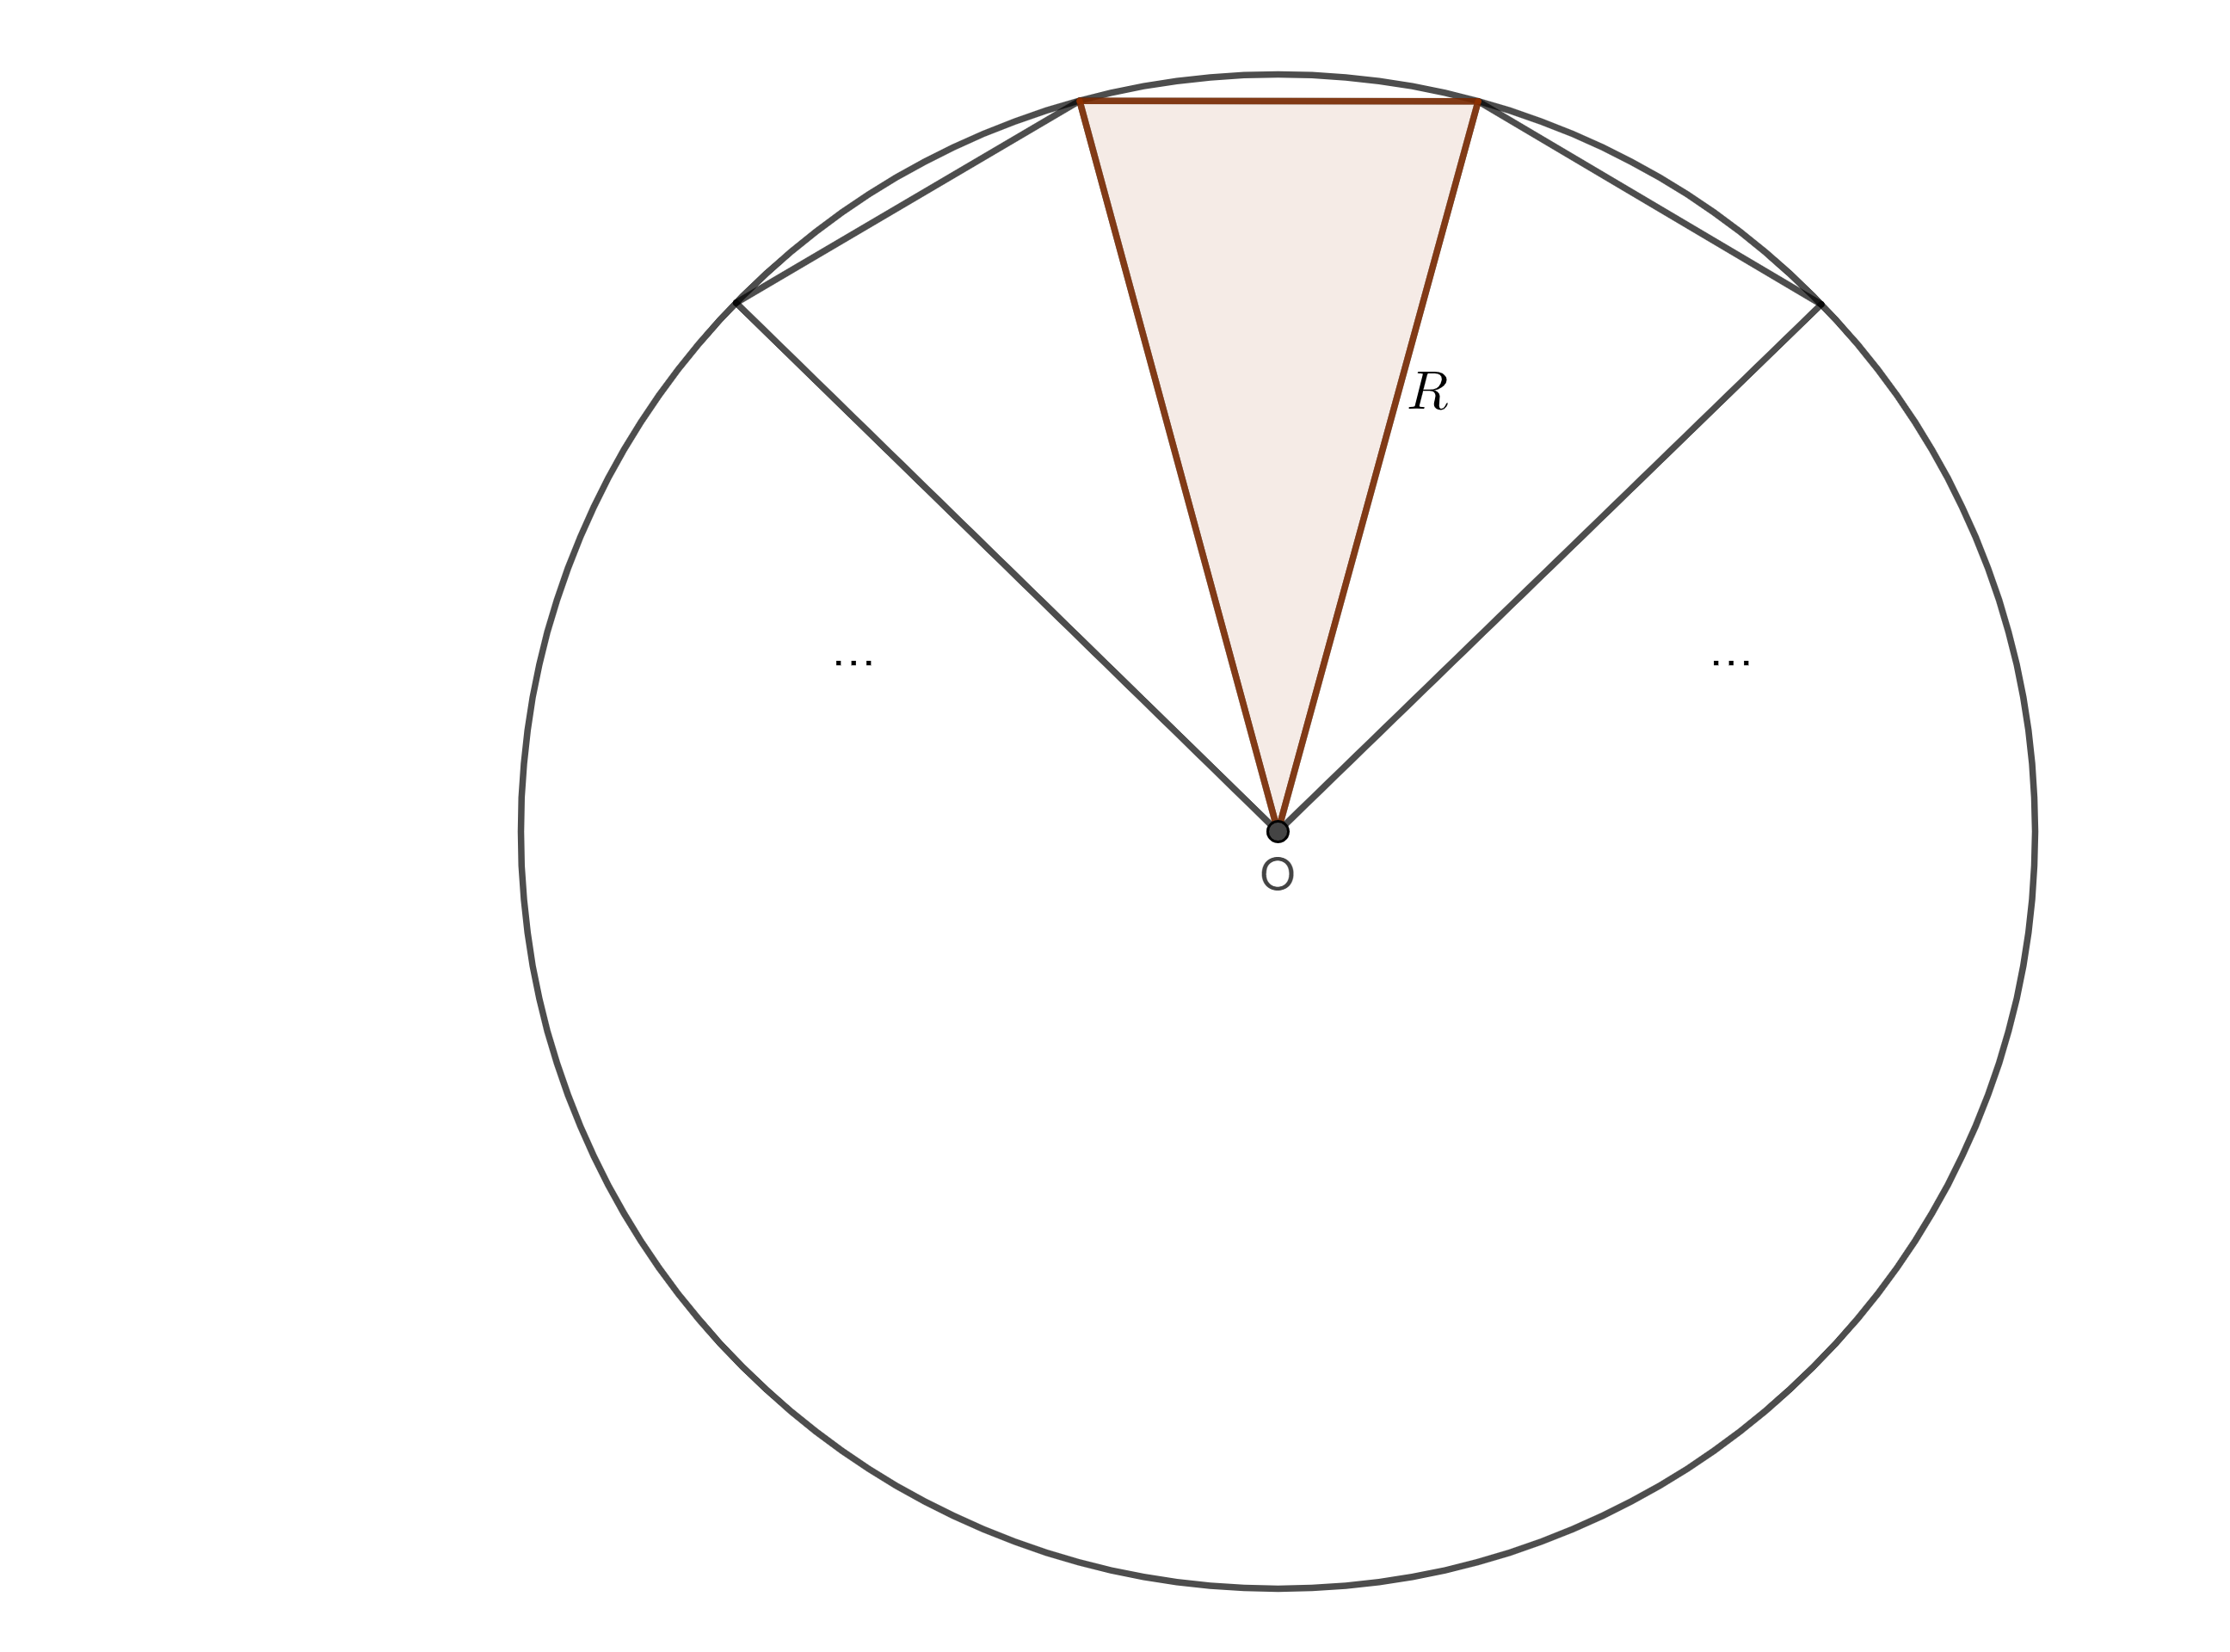
\includegraphics[width=0.4\linewidth]{img/circle.png}
  \vspace{0.5cm}
  \caption[Circle area approximation]{The area of a circle can be calculated by dividing it into equal isosceles triangles. As the number of triangles tends to infinity, the sum of bottom sides tends to the perimeter $2\pi R$ of the circle and the attitude of a triangle tends to $R$. Hence the area is $A=\dfrac{1}{2}(2\pi R)R=\pi R^2$.}
  \label{figure:circle}
\end{figure}

\begin{remark}
  These properties imply \textit{monotonicity}\index{monotonicity}, i.e. if $A\subset B$, then
  \begin{align}
    \mu(A)\le\mu(B).
  \end{align}
  Indeed, we have $$\mu(B)=\mu(A)+\mu(B\setminus A)\ge \mu(A).$$
\end{remark}

\begin{example}
  \begin{enumerate}
    \item []
    \item Consider the measurable space $(\RR, \mathcal{B}(\RR))  $. The function of taking the length of open intervals on the real line
          $$\mu((x,y))=|y-x|,\forall x,y\in\RR,$$
          which an assumption that $\mu(\varnothing)=0$, is a measure. Three properties of a measure are satisfied trivially.
    \item Consider the measurable space $(\RR, \mathcal{F})$, where $\mathcal{F}$ is any $\sigma$-algebra on $\RR$. Given $a\in\RR$. The indicator function $\mathbf{1}_a: \mathcal{F}\to\{0,1\}$ given by
          $$\begin{cases}
              \mathbf{1}_a(X)=1, & \text{ if } a\in X \\
              \mathbf{1}_a(X)=0, & \text{ otherwise }
            \end{cases}$$
          is a measure. We already have $\mathbf{1}_a(X)\ge0, \forall a\in X$. Let us check the other two properties of a measure for this function.
          \begin{itemize}
            \item Since $a\notin\varnothing$, we have $\mathbf{1}_a(\varnothing)=0$.
            \item For disjoints $X_1,X_2,\ldots$ it cannot be the case that there are two of them contain $a$. If $a\notin X_k,\forall k\in\mathbb{Z}^+$, then countable additivity holds since both sides are zero. Otherwise, if there exists $k\in \mathbb{Z}^+$ such that $a\in X_k$, then it follows that $$a\notin X_\ell, \forall \ell\ne k,$$ implying both sides are one.
          \end{itemize}
  \end{enumerate}
\end{example}

Given measure spaces $(\Omega,\mathcal{F},\mu)$ and $(\Gamma,\mathcal{G},\nu)$, we also concern about which pair $(\omega,\gamma)\in\Omega\times\Gamma$ that can be measured and how to measure them.

\begin{definition}
  Let $(\Omega,\mathcal{F},\mu)$ and $(\Gamma,\mathcal{G},\nu)$ be measure spaces. The product $\sigma$-algebra $\mathcal{F}\otimes\mathcal{G}$ on $\Omega\times\Gamma$ is given by
  $$\mathcal{F}\otimes\mathcal{G}=\mathcal{U}(\{A\times B\,|\, A\in\mathcal{F},B\in\mathcal{G}\}).$$
\end{definition}

\begin{definition}
  Let $(\Omega,\mathcal{F},\mu)$ and $(\Gamma,\mathcal{G},\nu)$ be measure spaces. The product measure $\lambda(A\times B)$ on $\mathcal{F}\otimes\mathcal{G}$, where $A\in\mathcal{F},B\in\mathcal{G}$ is given by
  $$\lambda(A\times B)=\mu(A)\nu(B)$$
\end{definition}

\begin{example}
  The measure of area $\mu$ in a two-dimensional space can be thought of as the product of two identical measures of length $\lambda$ in a one-dimensional space. Given two intervals $[a,b]$ and $[c,d]$, the equality
  $$\mu([a,b]\times [c,d])=\lambda([a,b])\cdot\lambda([c,d]),$$
  meets our intuition about the area of a rectangle. Here it is also suggests that a rectangle with one size to be zero has area measure zero.
\end{example}

\begin{definition}
  Given two measurable spaces $(\Omega, \mathcal{F})$ and $(\Gamma,\mathcal{G})$. A function $f:\Omega\to\Gamma$ is said to be measurable $\mathcal{F}\to\mathcal{G}$ if
  $$f^{-1}(A)\in\mathcal{F},\forall A\in \mathcal{G}.$$
\end{definition}

\subsubsection{Lebesgue Integral}
The Lebesgue integral extends the Riemann integral. If a function is Riemann-integrable, its Riemann integral equals its Lebesgue integral. However, Lebesgue integrals can handle functions not Riemann-integrable. This extension simplifies the formulation of theorems in probability, unifying discrete and continuous cases. The Riemann integral faces a limitation, demonstrated as follows.

The Fundamental Theorem of Calculus tells us that the limit $(\ref{equation:riem})$ exists and equals $F(b)-F(a)$, where $F$ is an anti-derivative of $f$. Geometrically, the integral coincides with the area of the region bounded by the horizontal axis and $f$, from $a$ to $b$. Challenges arise in higher dimensions due to partition definition. For example, if we decide to divide the integrating region $\Omega$ into boxes $\{B_k\}_{k=0}^\infty$ i.e. the Cartesian product of intervals, we must prove that the region can be approximated by the union of the boxes. Moreover, a selection of a point $\tau_k\in B_k$ results in a limit similarly to (\ref{equation:riem}), and we have to prove that all limits are equal.

The mathematician Henri Lebesgue came up with a new approach to approximate this area, or higher dimensional volumes, as illustrated in Figure $\ref{figure:schilling}$ in the case $d=1$. Suppose that $f$ is bounded on $[a,b]$. Consider partitions $$P^n=\left\{\inf\limits_{x\in K} f=t^n_0<t^n_1<\ldots<t^n_{m_n}=\sup\limits_{x\in K} f\right\}, n\in\mathbb{N}$$ such that $|P^n|\to 0$ as $n\to\infty$. For each $k\in\{0,\ldots,m_n-1\}$, there exists a set

\begin{figure}
  \centering
  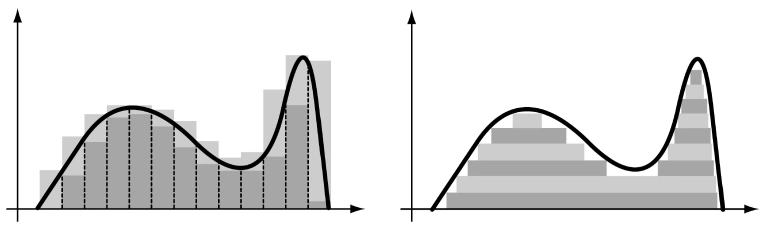
\includegraphics[width=0.75\linewidth]{img/riemann-vs-lebesgue.png}
  \vspace{0.5cm}
  \caption[Riemann and Lebesgue approximations]{Riemann and Lebesgue approximations \cite{schilling2017measures}}
  \label{figure:schilling}
\end{figure}



$$L_k^n=\{x\in\mathbb{K} \,|\, t_k^n\le f(x)\le t_{k+1}^n\}.$$

Let $\mu:2^{[a,b]}\to[0,\infty]$ be a measure for the length of each $L_k^n$, then
\begin{equation}
  I_n=\sum\limits_{k=0}^{m_n-1}(t_{k+1}-t_k)\mu(L_k^n)
\end{equation}

can be used as an approximation of the area under $f$. The measure for the length, area and volume of some subsets of $\RR$, $\RR^2$, $\RR^3$ and so on, is called \textit{Lebesgue measure}. The Lebesgue measure unifies Lebesgue integral and Riemann integral. Moreover, we can define Lebesgue integral for any measure rather than Lebesgue measure. Note that, each $L^n_k$ is $\mu$-measurable means that $f^{-1}([t_k^n, t^n_{k+1}])$ is $\mu$-measurable. Therefore, the function $f$ is required to be measurable $\mathcal{B}(\RR^d)\to\mathcal{B}(\RR)$. Let us formally develop Lebesgue integral for a general function $f:\Omega\to\RR$ as follows.

\begin{definition}
  Let $(\Omega, \mathcal{F}, \mu)$ be a measure space and $$A_1,\ldots,A_n\in\mathcal{F}.$$ A \index{step function} step function (simple function, elementary function) $f$ has the form
  \begin{equation}
    f(x)=\sum\limits_{i=1}^nc_i\mathbf{1}_{A_i}(x),
  \end{equation}
  where $c_1,\ldots,c_n$ are real constants.
\end{definition}

Since
$$\mathbf{1}_{A_i\cup A_j} = \mathbf{1}_{A_i} + \mathbf{1}_{A_j} - \mathbf{1}_{A_i\cap A_j},$$
we can choose $A_1,\ldots,A_n$ to be pairwise disjoint. For a step function $f$, if $x\in A_i\subset\mathcal{F}$, then we can think of $x$ as contributing to the element $c_i\mathbf{1}_{A_i}(x)$, hence we may define the Lebesgue integral of $f$ as
$$\mathcal{I}(f)=\sum\limits_{i=1}^nc_i\mu(A_i).$$
However, some $c_i, 1\le i\le n$ are positive and some are negative, make it not a convenient way, especially for later extension requiring $n\to\infty$, where we cannot specify clearly when the sum is finite. Therefore, we have to consider the domain of $f$ where the value of $f$ is non-negative, and otherwise.

\begin{definition}
  Let $f$ be a step function
  \begin{equation}
    \label{equation:step:pos}
    f(x)=\sum\limits_{i=1}^nc_i\mathbf{1}_{A_i}(x),
  \end{equation}
  where $c_i\ge0, 1\le i\le n$. The Lebesgue integral of $f$ is defined as
  $$\mathcal{I}(f)=\sum\limits_{i=1}^nc_i\mu(A_i).$$
\end{definition}

Any non-negative function $f$ on $\Omega$ i.e.$f(x)\ge 0,\forall x\in\Omega$ has a representation (\ref{equation:step:pos}). Indeed, as shown before, we can choose $A_i, 1\le i\le n$ to be pairwise disjoint. Suppose that there is $j\in\{1,\ldots,\}$ such that $c_j<0$, we take $x\in A_j$. Then $f(x)=c_j<0$, which contradicts to the non-negativity of $f$.

\begin{definition}
  Let $f:X\to[0,\infty)$ be measurable where $X\subset\Omega$. The Lebesgue integral of $f$ is defined as
  \begin{equation}
    \int\limits_{X}f\d \mu = \sup\left\{\mathcal{I}(h)\,|\, h\le f\right\}.
  \end{equation}
\end{definition}

\begin{definition}
  Let $f:X\to\RR$ be measurable where $X\subset\Omega$. Define
  $$f^+(x)=\begin{cases}
      f(x), & \text{ if } f(x)\ge 0 \\
      0,    & \text{ otherwise}
    \end{cases} \text{ and } f^-(x)=\begin{cases}
      f(x), & \text{ if } f(x)\le 0 \\
      0,    & \text{ otherwise.}
    \end{cases}$$

  The Lebesgue integral of $f$ is defined as
  \begin{equation}
    \int\limits_{X}f\d \mu = \int\limits_{X}f^+\d \mu - \int\limits_{X}(-f^-)\d \mu
  \end{equation}
  Then $f$ is said to be integrable or summable if $\int\limits_{X}f\d \mu<\infty$.
\end{definition}

To finish this section, we introduce $L^p$ space, an important class of spaces in analysis. Many later theorems in stochastic processes are proved in these spaces.

\begin{definition}
  Let $(\Omega,\mathcal{F},\mu)$ be a measure space, $f:\Omega\to\RR^m$ and $p\ge 1$. We define the $L^p(\mu)$-norm of $f$ (with respect to $\mu$) by
  $$\|f\|_{L^p(\mu)}=\left(\int\limits_\Omega \|f(\omega)\|^p_p\d \mu\right)^\frac{1}{p}.$$
  If $p=\infty$, define
  $$\|f\|_{L^\infty(\mu)}=\sup\{\|f(\omega)\|_p\}.$$
  Denote by $L^p(\mu)$ the vector space of all functions $f$ such that $\|f\|_{L^p}<\infty$.
\end{definition}

If there exist non-disjoint $A_i$ and $A_j$, we rewrite
$$c_i\mathbf{1}_{A_i}(x) + c_j\mathbf{1}_{A_j}(x) = c_i\mathbf{1}_{A_i\setminus A_j}(x) + (c_i+c_j)\mathbf{1}_{A_i \cap A_j}(x) + c_j\mathbf{1}_{A_j\setminus A_i}(x),$$
to achieve a disjoint family.

If there exist $c_i = c_j$, we rewrite
$$c_i\mathbf{1}_{A_i}(x) + c_j\mathbf{1}_{A_j}(x) = (c_i+c_j)\mathbf{1}_{A_i}(x) + c_j\mathbf{1}_{A_j\setminus A_i}(x).$$

Then the attained subset of $\RR$ is disjoint. Let us abuse the original notation
$$f(x)=\sum\limits_{n=1}^N c_n\mathbf{1}_{A_n}(x)$$
for this new representation. For each $A_n, n\in\{1,\ldots,N\}$, choose $x_n\in A_n$. We have $f(x_n) = c_n > 0$.


% \section{Predominant Diffusion Models}

% \subsection{Denoising Score Matching}
% Score-based generative modeling aims to approximate a probability distribution $p_{\text{data}}(\xbf)$ through its \textit{score function} $\nabla\log_{\xbf} p_{\text{data}}(\xbf)$ \cite{hyvarinen2005estimation}. Given observations $\{\xbf_1,\ldots,\xbf_N\}\subset\RR^d$, a basic method that is also highly intuitive is to model the dataset by a distribution $p(\xbf;\theta)$ and maximize the log-likelihood function

% \begin{equation}
%     \L(\theta)=\log\prod\limits_{i=1}^Np(\xbf_i;\theta).
% \end{equation}

% The problem is that real-life distribution, such as the CelebA dataset \cite{liu2015faceattributes}, are often highly complicated. Therefore, if we decide to model by a well-know distribution or a mixture of them, it may be not flexible enough. We can solve this problem by choosing any integrable function $f(\xbf,\theta)$ and let
% \begin{equation} p(\xbf;\theta)=\dfrac{f(\xbf;\theta)}{Z_\theta},
% \end{equation}

% where $Z_\theta=\int_{\xbf\in\RR^d}f(\xbf,\theta)\d \xbf$ is the \textit{normalizing constant}. However, as $f$ is a complicated function, $Z_\theta$ is usually intractable, especially in high-dimension. This is why score-based modeling is introduced, as the normalizing constant can now be ignored,
% \begin{align*}
%     \nabla_\xbf\log p_{\text{data}}(\xbf)
%     &\approx \nabla_\xbf\log p(\xbf;\theta)\\
%     &=\nabla_\xbf\log\dfrac{f(\xbf;\theta)}{Z_\theta}\\
%     &=\nabla_\xbf\log f(\xbf;\theta)-\nabla_\xbf\log Z_\theta = \nabla_\xbf\log f(\xbf;\theta),
% \end{align*} 
% since $Z_\theta$ does not depend on $\xbf$. In particular, the loss function is the divergence between the two score function of the real distribution and our approximating one,
% \begin{align}
% \label{equation:score-difference}
%     \L=\dfrac{1}{2}\EE_{p_{\text{data}}}[\|\nabla_\xbf\log p(\xbf,\theta)-\nabla_\xbf\log p_{\text{data}}(\xbf)\|^2_2].
% \end{align}

% Moreover, Hyvärinen \cite{hyvarinen2005estimation} proved that $\hat{\theta}$ can be estimated based on the observations under some regularity conditions.

% \begin{theorem}
% \label{theorem:score}
% Let 
% \begin{equation}
% \mathbf{s}_\theta(\xbf):=\nabla_\xbf\log p(\xbf,\theta)
% \end{equation} be a trainable score network. The objective function in \ref{equation:score-difference} can be expressed in the form
%     \begin{align}
%         \L(\theta) = \EE_{p_{\text{data}}}\left[\mathrm{tr}(\nabla_\xs_\theta(\xbf))+\dfrac{1}{2}\|\mathbf{s}_\theta(\xbf)\|^2_2\right]
%     \end{align}
%     up to constant difference, under some regularity conditions
%     \begin{enumerate}
%         \item The probability density distributions are differentiable.
%         \item For a probability density distribution $p(\xbf)$, $\lim\limits_{\|\xbf\|\to\infty}\nabla_\xbf p(\xbf) = \mathbf{0}$.
%     \end{enumerate}
% \end{theorem}

% One might wonder if the optimal parameter $\hat{\theta}=\argmin\limits_\theta\L(\theta)$ also makes the estimated distribution $p(\xbf,\hat{\theta})$ coincide with the unknown distribution $p_{\text{data}}(\xbf)$.  Hyvärinen also introduced a theoretical result to answer this question, as in the following theorem.

% \begin{theorem}
%     \label{theorem:thetahat}
%     Suppose that $p_{\text{data}}(\xbf)=p(\xbf,\hat{\theta})$ for a unique parameter $\hat{\theta}$. Then, $\L(\theta)=0$ if and only if $\theta=\hat{\theta}$.
% \end{theorem}

% Due to the complex architecture of the network $s_\theta(\xbf)$, it is not always possible to compute $\mathrm{tr}(\nabla_\xbf\mathbf{s}_\theta(\xbf))$ in practice. \textit{Denoising score matching} technique completely circumvents the computation of $\mathrm{tr}(\nabla_\xbf\mathbf{s}_\theta(\xbf))$ \cite{vincent2011connection}. Denote $q_\sigma(\tilde{\xbf}|\xbf)$ a prescribe transition with respect to $x\sim p_{\text{data}}$ and a scheduled noise value $\sigma$. DSM employs the score function $\mathbf{s}_\theta(\tilde{\xbf})$ of the perturbed data distribution given by
% \begin{equation}
% q_\sigma(\tilde{\xbf})=\int\limits_{\xbf\in\RR^d}q_\sigma(\tilde{\xbf}|\xbf)p_{\text{data}}(\xbf)\d \xbf.
% \end{equation}

% Then, the loss function (\ref{equation:denoise-loss}) becomes

% \begin{equation}
%     \label{equation:denoise-loss}
%     \L(\theta, \sigma)=\dfrac{1}{2}\EE_{\xbf\sim p_{\text{data}}(\xbf), \tilde{\xbf}\sim q_\sigma(\tilde{\xbf}|\xbf)}\left[\left\|\mathbf{s}(\mathbf{\tilde{x}})-\nabla_{\tilde{\xbf}}q_\sigma(\tilde{\xbf}|\xbf)\right\|_2^2\right].
% \end{equation}
% If we employ a Gaussian kernel for the transition $q_\sigma(\tilde{\xbf}|\xbf):=\N(\xbf;\tilde{\xbf},\sigma^2I_d)$, then we can express (\ref{equation:denoise-loss}) as
% \begin{equation}
%     \label{equation:denoise-loss-gaussian}
%     \L(\theta, \sigma)=\dfrac{1}{2}\EE_{\xbf\sim p_{\text{data}}(\xbf), \tilde{\xbf}\sim q_\sigma(\tilde{\xbf}|\xbf)}\left[\left\|\mathbf{s}(\mathbf{\tilde{x}})+\dfrac{\tilde{\xbf}-\xbf}{\sigma^2}\right\|_2^2\right],
% \end{equation}
% where we use
% \begin{align*}
% \nabla_{\tilde{\xbf}}q_\sigma(\tilde{\xbf}|\xbf)
% &=\nabla_{\tilde{\xbf}}\log\left\{\dfrac{1}{\sqrt{\d et(2\pi\sigma^2 I_d)}}\exp\left[-\dfrac{1}{2\sigma^2}(\mathbf{\tilde{x}}-\xbf)^\top(\mathbf{\tilde{x}}-\xbf)\right]\right\}\\
% &=\nabla_{\tilde{\xbf}}\left[-\dfrac{1}{2\sigma^2}(\mathbf{\tilde{x}}-\xbf)^\top(\mathbf{\tilde{x}}-\xbf)\right]\\
% &=-\dfrac{\mathbf{\tilde{x}}-\xbf}{\sigma^2}.
% \end{align*}

% Since $\mathbf{\tilde{x}}\in q_\sigma(\tilde{\xbf}|\xbf)$, we have $\mathbf{\tilde{x}}=\xbf+\sigma\bm{\epsilon}$, for $\bm{\epsilon}\in\N(\mathbf{0}, I_d)$. Therefore, if we let $\bm{\epsilon}_\theta(\mathbf{\tilde{x}}):=-\sigma\mathbf{s}_\theta(\mathbf{\tilde{x}})$, we obtain an equivalent form of (\ref{equation:denoise-loss}) as

% \begin{equation}
%     \L(\theta, \sigma)=\dfrac{1}{2\sigma^2}\EE_{\xbf\sim p_{\text{data}}(\xbf), \tilde{\xbf}\sim q_\sigma(\tilde{\xbf}|\xbf)}\left[\left\|\bm{\epsilon}_\theta(\mathbf{\tilde{x}})-\bm{\epsilon}\right\|_2^2\right],
% \end{equation}

% in which $\bm{\epsilon}_\theta(\mathbf{\tilde{x}})$ can be regarded is a \textit{noise prediction} model that predicts how much noise is added into $\xbf$ to construct the perturbed $\mathbf{\tilde{x}}$. On the other hand, if we set $D_\theta(\mathbf{\tilde{x}}) := \sigma^2\mathbf{s}_theta(\mathbf{\tilde{x}})+\mathbf{\tilde{x}}$, (\ref{equation:denoise-loss-gaussian}) becomes

% \begin{equation}
%     \L(\theta, \sigma)=\dfrac{1}{2\sigma^4}\EE_{\xbf\sim p_{\text{data}}(\xbf), \tilde{\xbf}\sim q_\sigma(\tilde{\xbf}|\xbf)}\left[\left\|D_\theta(\mathbf{\tilde{x}})-\xbf\right\|_2^2\right],
% \end{equation}

% in which $D_\theta(\mathbf{\tilde{x}})$ is regarded as a \textit{data prediction} model that denoises the perturbed $\mathbf{\tilde{x}}$ to be close to the clean data $\xbf$. This interpretation results in the name DSM of this approach.

% \subsubsection*{Forward Process}

% Given a schedule set of noise levels $\{\sigma_i\}_{i=1}^N$, the denoise score matching models trained by Gaussian perturbed distributions $q_{\sigma_i}(\tilde{\xbf}|\xbf):=\N(\xbf;\tilde{\xbf},\sigma_i^2I_d)$ with $\xbf_0\sim p_{\text{data}}$ implies that

% \begin{equation}
%     \label{equation:perturbed}
%     \xbf_i = \xbf_0 + \sigma_i \bm{\epsilon}_i,
% \end{equation}
% where $\bm{\epsilon}_i\sim\N(\mathbf{0}, I_d)$. Then, we choose a Markov process $\{x_i\}_{i=1}^N$ which derives the perturbed distributions (\ref{equation:perturbed}). A straightforward idea is to select the transitions from $\xbf_{i-1}$ to $\xbf_i$ to be Gaussian distributions i.e.
% \begin{equation}
%     q(\xbf_i|\xbf_{i-1})=\N(\xbf_i;\xbf_{i-1}, \upsilon^2(\sigma_i,\sigma_{i-1})I_d),
% \end{equation}
% where $\epsilon_0=0$. This implies
% \begin{align*}
%     \xbf_i 
%     &= \xbf_{i-1} + \sqrt{\upsilon^2(\sigma_i,\sigma_{i-1})}\bm{\epsilon}_i\\
%     &= \xbf_{i-2} + \sqrt{\upsilon^2(\sigma_{i-1},\sigma_{i-2})}\bm{\epsilon}_{i-1} + \sqrt{\upsilon^2(\sigma_i,\sigma_{i-1})}\bm{\epsilon}_i\\
%     &= \cdots\\
%     &= \xbf_{0}+\sum\limits_{j=1}^{i}\sqrt{\upsilon^2(\sigma_j,\sigma_{j-1})}\bm{\epsilon}_j.
% \end{align*}

% The sum of zero-mean Gaussians $\sum\limits_{j=1}^{i}\sqrt{\upsilon^2(\sigma_j,\sigma_{j-1})}\bm{\epsilon}_j$ is again a zero-mean Gaussian, and its variance must be equal to that of $q(\xbf_i|\xbf_{i-1})$. Therefore,

% $$\sum\limits_{j=1}^{i}\sqrt{\upsilon^2(\sigma_j,\sigma_{j-1})}=\sigma_i^2, i\in\{1,\ldots,N\}.$$

% Solving this system of equations gives
% \begin{align*}
%     \upsilon^2(\sigma_1,\sigma_{0})&=\sigma^2_1,\\
%     \upsilon^2(\sigma_2,\sigma_{1})&=\sigma_2^2-\upsilon^2(\sigma_1,\sigma_{0})=\sigma_2^2-\sigma^2_1,\\
%     \upsilon^2(\sigma_3,\sigma_{2})&=\sigma_3^2-\upsilon^2(\sigma_2,\sigma_{1})-\upsilon^2(\sigma_1,\sigma_{0})\\
%     &=\sigma_3^2-(\sigma_2^2-\sigma^2_1)-\sigma^2_1\\
%     &=\sigma_3^2-\sigma_2^2\\
%     &\vdots\\
%     \upsilon^2(\sigma_N,\sigma_{N-1})&=\sigma^2_N-\sigma^2_{N-1}.
% \end{align*}

% Thus, we arrive at
% \begin{equation}
%     \xbf_i=\xbf_{i-1}+\sqrt{\sigma_i^2-\sigma_{i-1}^2}\bm{\epsilon}_{i-1}.  
% \end{equation}

% Now, take $\{\sigma_t\}_{t\ge0}$ and an arbitrary time step $\Delta t\ge0$, we have
% \begin{align*}
%     \xbf_{t+\Delta t}-\xbf_{t}
%     &=\sqrt{\sigma_{t+\Delta t}^2-\sigma_{t}^2}\bm{\epsilon}_{t}\\
%     &=\sqrt{\dfrac{\sigma_{t+\Delta t}^2-\sqrt{\sigma_t}^2}{\Delta t}}\Delta t\cdot\bm{\epsilon}_{t}\\
%     &=\sqrt{\dfrac{\sigma_{t+\Delta t}^2-\sigma_t^2}{\Delta t}}(\mathbf{\mathbf{W}}_{t+\Delta t}-\mathbf{W}_{t}),
% \end{align*}
% where $\mathbf{W}_t$ is the $n$-dimensional Wiener process. Taking the limit when $\Delta\to 0$ yields an SDE
% \begin{align}
%     \d \xbf_{t}=\sqrt{\dfrac{\d \sigma^2(t)}{\d t}}\d \mathbf{W}_{t}.
% \end{align}

% This is the continuous-time setting of DSM.


% \subsubsection*{Reverse process}

% After the score function $\mathbf{s}_\theta(\xbf)$ is trained well enough, if we have the analytic form $\mathbf{s}_\theta(\xbf)=\nabla_\xp(\xbf,\theta)$, we can retrieve $p(\xbf,\theta)$ as an approximation of $p_{\text{data}}(\xbf)$, according to Theorem (\ref{theorem:thetahat}). However, if
% we do not have access to the closed form of the estimated score $\mathbf{s}_\theta(\xbf)$, we can otherwise leverage Langevin dynamics to sample, \cite{welling2011bayesian} in which only the score function is required. Specifically, we assume that $\tilde{\xbf}\sim\pi(\tilde{\xbf})$ where $\pi$ is a prior distribution. Langevin dynamics recursively computes
% \begin{equation}
%     \label{equation:langevin}
%     \tilde{\xbf}_t = \tilde{\xbf}_{t-1}+\dfrac{\delta}{2}\nabla_\xbf\log p(\tilde{\xbf}_{t-1}) + \sqrt{\delta}\bm{\epsilon}_t,
% \end{equation}
% where $\bm{\epsilon}_t\sim\N(\mathbf{0}, I_d)$. When $\delta\to0$ and $N\to\infty$ the distribution of $\tilde{\xbf}_N$ approaches $p_{\text{data}}$ under some regularity conditions \cite{welling2011bayesian}. By substituting the score network $\mathbf{s}_\theta(\xbf)$ into (\ref{equation:langevin}), we obtain an iterative update formula that can sample from p_data for very small $\delta$ and sufficiently large number of iterations $N$.

whose transition densities
satisfy the Markov property, i.e. for $i=1,\ldots,N$
\begin{equation}
  q(\xbf_i|\xbf_{i-1},\cdots,\xbf_0)=q(\xbf_i|\xbf_{i-1}).
\end{equation}
Along with Bayes' rule, we have
\begin{align*}
  q(\xbf_0,\xbf_1,\xbf_2)
   & = q(\xbf_0,\xbf_1)q(\xbf_2|\xbf_0,\xbf_1)                   \\
   & =q(\xbf_0)q(\xbf_1|\xbf_0)q(\xbf_2|\xbf_1)                  \\
  q(\xbf_0,\xbf_1,\xbf_2,\xbf_3)
   & = q(\xbf_0,\xbf_1,\xbf_2)q(\xbf_3|\xbf_0,\xbf_1,\xbf_2)     \\
   & =q(\xbf_0)q(\xbf_1|\xbf_0)q(\xbf_2|\xbf_1)q(\xbf_3|\xbf_2).
\end{align*}
Consequently,
\begin{equation} q(\xbf_0,\cdots,\xbf_N)=q(\xbf_0)\prod\limits_{i=1}^Nq(\xbf_i|\xbf_{i-1}).
\end{equation}

Now let $\{\beta_i\}_{i=1}^N\subset(0,1)^N$ be scheduled variances. The transition distribution in DDPM is

\begin{example}
  Given a set of 52 poker cards, each card has a rank between 1 and 13 and one of four suits. Randomly choose a card in the set, what is the probability of receiving a black five.
\end{example}

Let $X$ be the random variable indicating the rank of a card whose values coincide with the rank itself. Let $Y$ indicate the suit, whose values 1,2,3 and 4 for spade, club, tile and heart, respectively. The problem is to calculate the probability
$$P(X\in\{5\}, Y\in\{1,2\}).$$

More generally, one can answer questions on the probability of the form
$$P(X\in S_X, Y\in S_Y),$$
where $S_X\subset\{1,\ldots,13\}$ and $S_Y\subset\{1,\ldots,4\}$. This is the same as to come up with a \textit{joint} PMF $p_{X,Y}(x,y)$. Another type of questions can also be made, such as the probability of receiving a five \textit{given} that the chosen card is black. This can be regarded as a conditional PMF $p_{X|Y}(x,y)$. Before discussing the theorems, let us consider a continuous-case example.

\begin{example}
  In a population, we measure the weight and height of people, represented by random variables $X$ and $Y$. What is the probability that a people under $160\,cm$ weighed more than $60\,kg$?
\end{example}

\begin{definition}[Cumulative Distribution Function and Probability Density Function]
  Let $X=(X_1,\ldots, X_d)$ be a $d$-dimensional random variable.
  The cumulative distribution function (CDF) of $X$ is the function
  $$P_X:\RR^n\to [0,1],$$
  such that
  \begin{equation}
    P_X(x_1,\ldots,x_d)=\PP(X_1\le x_1,\ldots,X_d\le x_d).
  \end{equation}

  If there exists a function $p_X:\RR^n\to [0,1]$ such that
  $$P_X(x_1,\ldots,x_n)=\int\limits_{-\infty}^{x_1}\cdots\int\limits_{-\infty}^{x_n}p_X(x_1,\ldots,x_n)\d x_n\cdots\d x_1,$$
  then $X$ is said to be absolutely continuous\index{absolutely continuous}. We call $p_X$ the probability density function (PDF) of $X$, and denote by $X\sim p_X$.
\end{definition}

At timestep 0, the histogram indicates the distribution of pixel values in the input image, displaying an arbitrary pattern. Following the first forward step at timestep 1, the histograms for all three channels begin to exhibit a mixture of Gaussian patterns, likely representing a combination of two Gaussians.

% For a clearer understanding of the DDPM forward and backward processes, we conducted a straightforward experiment using an image sourced from Stable, Wikipedia, as shown in Figure \ref{figure:test-img}. In this experiment, we configured the processes by solving Stochastic Differential Equations (SDEs). The forward SDE takes the form
% \begin{equation}
%   \text{d}\xbf(t) = f(t)\xbf(t)\text{d}t + g(t)\text{d}\textbf{W}(t),
% \end{equation}
% where $f(t) := \frac{\text{d log}\alpha(t)}{\text{d}t} = \frac{\dot{\alpha(t)}}
%   {\alpha(t)}$ and $g(t) := \alpha(t)\sqrt{\frac{\text{d}[\sigma^2(t)]}{\text{d}t}} = \alpha(t)\sqrt{2\dot{\sigma}(t)\sigma(t)}$. The corresponding reverse SDE has the form
% \begin{equation}
%   \text{d}\xbf(t) = [f(t)\xbf(t) - g^2(t)\nabla_{\xbf}\log p_{t}(\xbf(t); t)]\text{d}t + g(t)d\textbf{W}(t)
% \end{equation}
% \begin{figure}[H]
%   \centering
%   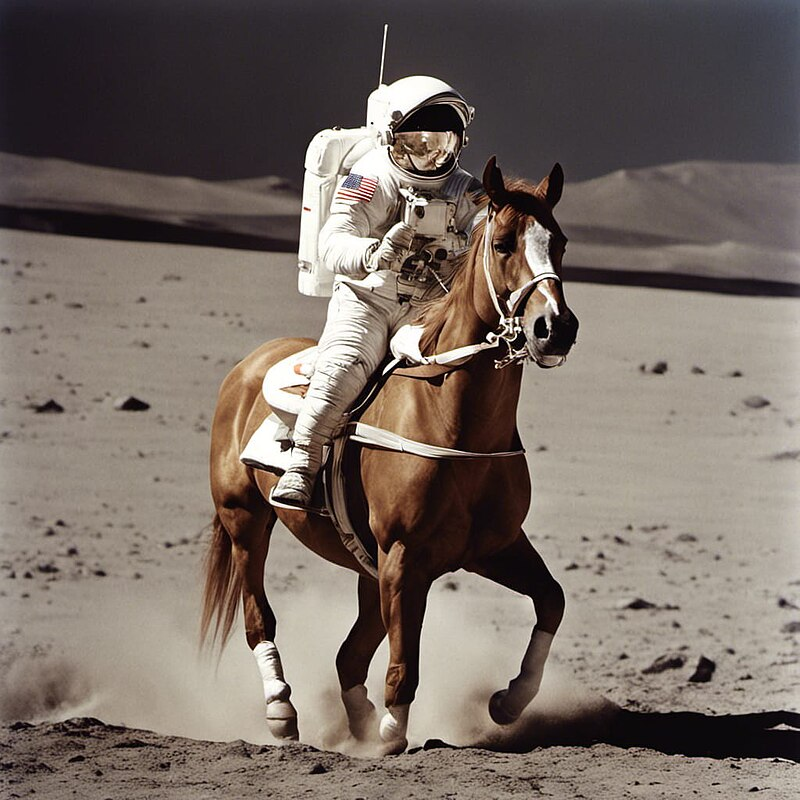
\includegraphics[width = 0.25\textwidth]{img/test_img.jpg}
%   \vspace{1cm}
%   \caption[A sample image to run DDPM]{A sample image to run DDPM with a size of $256 \times 256$\footnotemark}
%   \label{figure:test-img}
% \end{figure}
% \footnotetext{\href{https://en.wikipedia.org/wiki/Stable_Diffusion}{Stable Diffusion on Wikipedia}}

% With the forward and backward SDE definitions in place, we employed the DDPM setting outlined by Karras et al. \cite{karras2022elucidating}. To facilitate the implementation, we utilized the torchsde library\footnote{https://github.com/google-research/torchsde}, a Python library built on the torch framework. This library, developed by Google, supports the solving of Stochastic Differential Equations (SDEs). The results of our experiment are visualized in Figure \ref{figure:yangsong}.

% However, inpainting-based watermark removal methods are supposed to point out the watermark location in the image. Moreover, inpainting based methods completely erase the masked region, and the background context will be re-generated by the neural network other than re-using the texture from the input. Differently, in the task of watermark removal, the transparent watermark contains both background and foreground information. Ignoring background cures will destroy the original structure, gaining undesired results. The example of the Image Inpainting Method is shown in Figure \ref{figure:inpainting_1}.
% \begin{figure}[H]
%   \centering
%   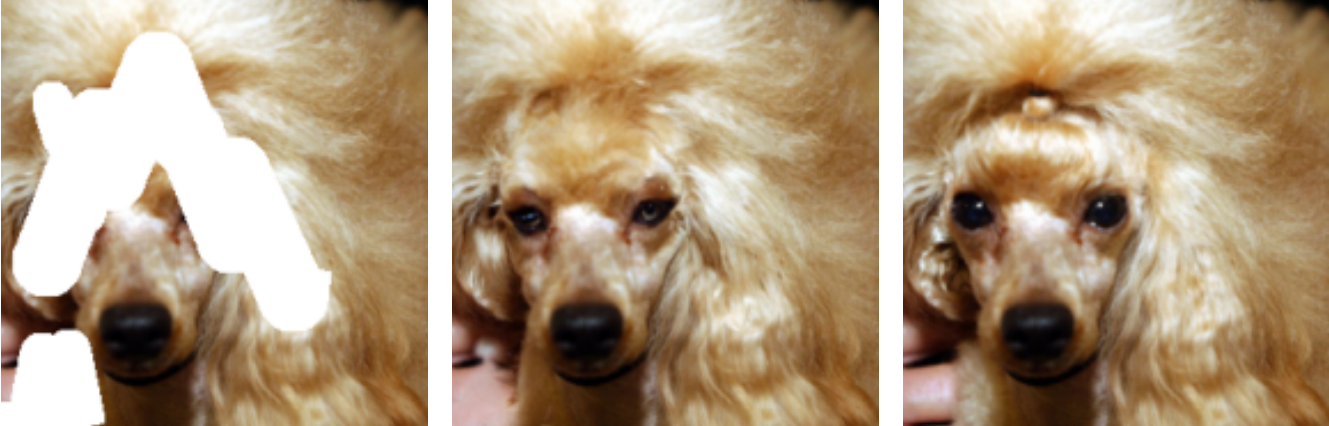
\includegraphics[width=0.75\linewidth]{img/inpainting_1.png}
%   \vspace{1cm}
%   \caption{Example of Image Inpainting methods}
%   \label{figure:inpainting_1}
% \end{figure}

Recently, which the introduction of Diffusion-based models, many researchers have utilized the generative ability of diffusion models to implement tasks on Image Inpainting. Diffusion and score-based generative models \cite{sohl2015deep} \cite{song2020score} have become potent conditional generative models, showcasing notable success in generating high-fidelity data \cite{dhariwal2021diffusion} \cite{rombach2022high} \cite{vahdat2021score}. These models operate by progressively transforming data into noise and learning score functions, often represented by neural networks, to reverse these processes \cite{anderson1982reverse}. This reversal enables the generation of data from noise. In recent studies, inpainting tasks have been considered as the restoration of a degraded image (masked image) to its clean counterpart (original image).

Generative processes can be adapted for image restoration by introducing degraded images as extra inputs to the score network \cite{saharia2022image} \cite{saharia2022palette}. This approach biases the processes towards generating corresponding intact images. Alternatively, if the mapping between clean and degraded images is known, the tasks can be reformulated as inverse problems. In this context, diffusion priors (Kawar et al., 2022 \cite{zhu2023denoising}; Wang et al., 2022 \cite{wang2022zero}) guide the restoration of the underlying clean signal from the degraded measurement.

In this project, we employ a diffusion-based method for the image inpainting task, known as the \textbf{Image-to-Image Schrödinger Bridge (I$^2$SB)}. This model belongs to a novel category of conditional diffusion models, proficient in learning fully nonlinear diffusion bridges connecting two domain distributions. It not only produces more interpretable generation but also demonstrates significant success in various restoration tasks, such as super-resolution, debluring, inpainting, and JPEG restoration.

Recently, the majority of the aforementioned diffusion models used for image restoration initiate their generative denoising processes with Gaussian white noise. However, Gaussian white noise possesses minimal or no structural information about the clean data distribution. While this approach is inherent in unconditional generation, it remains uncertain whether this default setup is optimal for image-to-image translation problems, particularly in image restoration. In cases where degraded images contain significantly more structural information than random noise, alternative setups might be worth exploring.

An alternative approach that capitalizes on the problem's structure involves initiating the generative processes directly from degraded images. This strategy entails constructing diffusion "bridges" between clean and degraded data distributions. This concept shares similarities with image-to-image translation Generative Adversarial Networks (GANs) as presented by Zhu et al. \cite{zhu2017unpaired} and Huang et al. \cite{huang2018multimodal}. The construction of these diffusion bridges often requires a new computational framework for reversing general diffusion processes.

\subsubsection*{Algorithm design}

We now then discuss practical designs for applying Theorem \ref{theo-dirac} to image restoration. Efficiently computing $X_t$ is crucial for training scalable diffusion models. However, directly obtaining it for I$^2$SB from the nonlinear SDE \ref{sb-fw} is impractical due to the nonlinear nature of its forward drift $\gradlog \Psi$, which is not explicitly constructed. Utilizing the linear SDE \ref{sb-fw-2} is also not a viable option, as the diffusion process in this equation does not converge to the terminal distribution ($p_\B(X_1|X_0)$) of I$^2$SB. Consequently, the high-probability regions induced by \ref{sb-fw-2} may be distant from the actual regions traversed by the generative processes. This challenge is addressed in the following result.

\begin{proposition}[Analytic posterior given boundary pair] \label{proposition:3}
  The posterior of {\ref{sb-fw}, \ref{sb-bw}} given some boundary pair $(\xbf_0, \xbf_1)$, provided $f := 0$, admits an analytic form:
  \begin{align*}
          & q(\xbf_t|\xbf_0, \xbf_1) = \N(\xbf_t; \mu_t(\xbf_0, \xbf_1), \Sigma_t), \numberthis \label{equation:prop3} \\
    \mu_t & = \frac{\bar{sigma}_t^2}{\bar{sigma}_t^2 + \sigma^2_t} \xbf_0 +
    \frac{\sigma^2_t    }{\bar{sigma}_t^2 + \sigma^2_t} \xbf_1,\quad
    \Sigma_t = \frac{\sigma_t^2 \bar{sigma}_t^2}{\bar{sigma}_t^2 + \sigma^2_t} \cdot I,
  \end{align*}
  where $\sigma^2_t {:=} \int_0^t \beta_\tau \d \tau$ and $\bar{sigma}^2_t {:=} \int_t^1 \beta_\tau \d \tau$ are variances accumulated from either sides.
  Further, this posterior marginalizes the recursive posterior sampling in DDPM \eqref{equation:ddpm_rev}:
  \begin{align*}
    q(\xbf_n|\xbf_0,\xbf_N) {=} {\int} \Pi_{k=n}^{N-1} p(\xbf_{k}|\xbf_0, \xbf_{k{+}1}) \d \xbf_{k{+}1}.
  \end{align*}
\end{proposition}

Proposition \ref{proposition:3} suggests that the analytic posterior of SB given a boundary pair $(\xbf_0, \xbf_1)$
is the marginal density induced by DDPM, $p(\xbf_{k}|\xbf_0^\epsilon, \xbf_{k{+}1})$, when $\xbf_0^\epsilon := \xbf_0$
and $\xbf_N \sim p_\B$.
Practically, this suggests that \textit{(i)} during training when $(\xbf_0, \xbf_1)$ are available from $p_\A(\xbf_0)$ and $p_\B(\xbf_1|\xbf_0)$, we can sample $\xbf_t$ directly from \eqref{equation:prop3} without solving any nonlinear diffusion as in prior SB models \cite{vargas2021solving}, and \textit{(ii)} during generation when only $\xbf_1\sim p_\B$ is given,
running standard DDPM starting from $\xbf_1$ induces the same marginal density of SB paths so long as the predicted $\xbf_0^\epsilon$ is close to $\xbf_0$. %
Therefore, the proposed sampling proposal in Equation \ref{equation:prop3} is both tractable and able to cover regions traversed by generative processes.

\textbf{Parameterization \& Objective$\quad$}
Since I$^2$SB requires no conditioning modules, we adopt the same network parameterization $\epsilon(\xbf_t,t;\theta)$ from SGM \cite{dhariwal2021diffusion}.
We can compute the score function for $\gradlog \Psihat(\xbf_t,t|\xbf_0) \equiv \gradlog~p^\text{\eqref{sb-fw-2}}(\xbf_t,t|\xbf_0)$, except $\xbf_t$ being drawn from \eqref{equation:prop3}.
This leads to
\begin{align} \label{equation:obj}
  \|
  \epsilon(\xbf_t,t; \theta) - \frac{\xbf_t {-} \xbf_0}{\sigma_t}
  \|
\end{align}

With the compilation of the theories provided here, we can now establish the algorithm for both training and sampling in the I$^2$SB model.

\begin{algorithm}[H]
  \caption{Training}
  \label{algorithm:train}
  \begin{algorithmic}[1]
    \STATE {\bfseries Input:} clean $p_\A(\cdot)$ and degraded $p_\B(\cdot|\xbf_0)$ datasets
    \REPEAT
    \STATE $t\sim\U([0,1])$, $\xbf_0 \sim p_\A(\xbf_0)$, $\xbf_1 \sim p_\B(\xbf_1|\xbf_0)$
    \STATE $\xbf_t \sim q(\xbf_t|\xbf_0,\xbf_1)$ according to \eqref{equation:prop3}
    \STATE Take gradient descent step on $\epsilon(\xbf_t,t;\theta)$ using \eqref{equation:obj}
    \UNTIL{converges}
  \end{algorithmic}
\end{algorithm}

\begin{algorithm}[H]
  \caption{Generation}
  \label{algorithm:sample}
  \begin{algorithmic}[1]
    \STATE {\bfseries Input:} $\xbf_N \sim p_\B(\xbf_N)$, trained $\epsilon(\cdot,\cdot; \theta)$
    \FOR{$n=N$ {\bfseries to} $1$}
    \STATE Predict $\xbf_0^\epsilon$ using $\epsilon(\xbf_n, t_n; \theta)$
    \STATE $\xbf_{n-1} \sim p(\xbf_{n-1} | \xbf_0^\epsilon, \xbf_n)$ according to DDPM \eqref{equation:ddpm_rev}
    \ENDFOR
    \STATE {\bfseries return} $\xbf_0$
  \end{algorithmic}
\end{algorithm}
